\documentclass[10pt,openany]{book}
\usepackage{iftex}
\ifPDFTeX
\usepackage[utf8]{inputenc}
\DeclareUnicodeCharacter{2212}{\ensuremath{-}}
\DeclareUnicodeCharacter{2192}{\ensuremath{\to}}
\DeclareUnicodeCharacter{03B1}{\ensuremath{\alpha}}
\DeclareUnicodeCharacter{2248}{\ensuremath{\approx}}
\DeclareUnicodeCharacter{00D7}{\ensuremath{\times}}
\DeclareUnicodeCharacter{0394}{\ensuremath{\Delta}}
\DeclareUnicodeCharacter{2074}{\ensuremath{^4}}
\fi
\usepackage[T1]{fontenc}
\usepackage{lmodern}
\AtBeginDocument{\normalfont\DeclareFontShape{T1}{lmr}{bx}{sc}{<->ssub*lmr/m/sc}{}}
\usepackage[spanish,es-nodecimaldot]{babel}
\spanishplainpercent
\AtBeginDocument{\spanishdeactivate{"~<>}}
\usepackage[a4paper,margin=2.5cm,headheight=14pt]{geometry}
\usepackage{needspace}
\usepackage{amsmath,amssymb,mathtools,booktabs,array,longtable,graphicx,xcolor,tikz,enumitem,microtype,titlesec,fancyhdr}
\usepackage[breakable,skins]{tcolorbox}
\usepackage[labelfont=bf]{caption}
\usepackage[hyphens]{url}
\usepackage[hidelinks,unicode,hypertexnames=false]{hyperref}
\definecolor{studiumInk}{RGB}{20,44,64}
\definecolor{studiumBlue}{RGB}{24,74,130}
\definecolor{studiumCyan}{RGB}{0,184,205}
\definecolor{studiumLight}{RGB}{232,240,250}
\definecolor{studiumWorkedBack}{RGB}{255,244,230}
\definecolor{studiumWorkedFrame}{RGB}{138,78,12}
\definecolor{studiumCheckBack}{RGB}{243,236,248}
\definecolor{studiumCheckFrame}{RGB}{96,48,130}
\titleformat{\chapter}[display]{\normalfont\filright}{\large\mdseries\scshape\chaptertitlename\ \thechapter}{1ex}{\normalfont\huge\bfseries}
\titlespacing*{\chapter}{0pt}{2.5ex plus 1ex minus .2ex}{2.3ex}
\titleformat{name=\chapter,numberless}[display]{\normalfont\filright}{}{0pt}{\normalfont\huge\bfseries}
\titleformat{\section}{\Large\bfseries}{\thesection}{.8em}{}
\titleformat{\subsection}{\large\bfseries}{\thesubsection}{.7em}{}
\makeatletter
\renewcommand*\l@section{\@dottedtocline{1}{1.5em}{3.5em}}
\renewcommand*\l@subsection{\@dottedtocline{2}{3.8em}{5em}}
\makeatother
\setcounter{secnumdepth}{2}\setcounter{tocdepth}{2}
\setlength{\parindent}{1.5em}\setlength{\parskip}{3pt plus .5pt}
\setlength{\emergencystretch}{1.5em}\raggedbottom
\setlist{itemsep=2pt,topsep=4pt,leftmargin=*}
\setlist[description]{style=nextline,leftmargin=0pt,labelwidth=0pt,labelindent=0pt}
\allowdisplaybreaks[2]
\graphicspath{{figures/}}
\newcommand{\Raire}{287.05287}
\newcommand{\gzero}{9.80665}
\tcbset{studiumcommon/.style={breakable,boxrule=.65pt,arc=.7pt,left=1.7mm,right=1.7mm,top=1.3mm,bottom=1.3mm,before skip=10pt,after skip=10pt,fonttitle=\bfseries}}
\newtcolorbox{studiumworked}[1]{studiumcommon,colback=studiumWorkedBack,colframe=studiumWorkedFrame,colbacktitle=studiumWorkedFrame,coltitle=white,title={#1}}
\newcommand{\objetivos}[1]{\par\noindent\textbf{Objetivos de aprendizaje.} \textit{#1}\par\medskip}
\newcommand{\caja}[2]{\begin{tcolorbox}[studiumcommon,colback=studiumLight,colframe=studiumBlue,colbacktitle=studiumBlue,coltitle=white,title={#1}]#2\end{tcolorbox}}
\newcommand{\resumen}[1]{\begin{tcolorbox}[studiumcommon,colback=studiumCheckBack,colframe=studiumCheckFrame,colbacktitle=studiumCheckFrame,coltitle=white,title=Resumen]#1\end{tcolorbox}}
\newcommand{\figura}[2]{\begin{figure}[tbp]\centering\includegraphics[width=.83\linewidth]{#1.pdf}\caption{#2}\label{fig:#1}\end{figure}\noindent La figura~\ref{fig:#1} ofrece una representación del modelo discutido.}
\pagestyle{fancy}\fancyhf{}
\fancyhead[LE]{\small\thepage\hspace{1.5em}\mdseries\scshape\nouppercase{\leftmark}}
\fancyhead[RO]{\small\mdseries\scshape\nouppercase{\rightmark}\hspace{1.5em}\thepage}
\renewcommand{\headrulewidth}{.4pt}\renewcommand{\footrulewidth}{0pt}
\fancypagestyle{plain}{\fancyhf{}\fancyfoot[C]{\small\thepage}\renewcommand{\headrulewidth}{0pt}}

% Retícula Studium unificada: cabecera blanca, fotografía a sangre y bloque azul.
\addto\captionsspanish{\renewcommand{\contentsname}{Índice}\renewcommand{\tablename}{Cuadro}\renewcommand{\listtablename}{Índice de cuadros}}
\numberwithin{equation}{chapter}
\let\cleardoublepage\clearpage
\fancyfoot[R]{\scriptsize\sffamily\color{studiumInk}En revisión}
\renewcommand{\chaptermark}[1]{\markboth{Capítulo \thechapter.\ #1}{}}
\renewcommand{\sectionmark}[1]{\markright{\thesection\ #1}}
\definecolor{studiumTipBack}{RGB}{232,244,236}
\definecolor{studiumTipFrame}{RGB}{27,107,58}
\newcommand{\consejo}[2]{\begin{tcolorbox}[studiumcommon,colback=studiumTipBack,colframe=studiumTipFrame,colbacktitle=studiumTipFrame,coltitle=white,title={#1}]#2\end{tcolorbox}}
\newcommand{\estado}{Edición íntegra de estudio. Pendiente de revisión experta independiente.}
\newcommand{\portada}[3]{%
\hypersetup{pageanchor=false}
\begin{titlepage}\thispagestyle{empty}
\begin{tikzpicture}[remember picture,overlay,x=1bp,y=-1bp]
\begin{scope}[shift={(current page.north west)}]
\clip (0,0) rectangle (595.276,841.89);
\fill[white] (0,0) rectangle (595.276,841.89);
% Hero fotografico preencuadrado en la reticula de la coleccion (mismo
% borde superior y mismo bloque inferior que Teoria de Estructuras/Fluidos).
\node[anchor=north west,inner sep=0pt,outer sep=0pt] at (0,89.5)
  {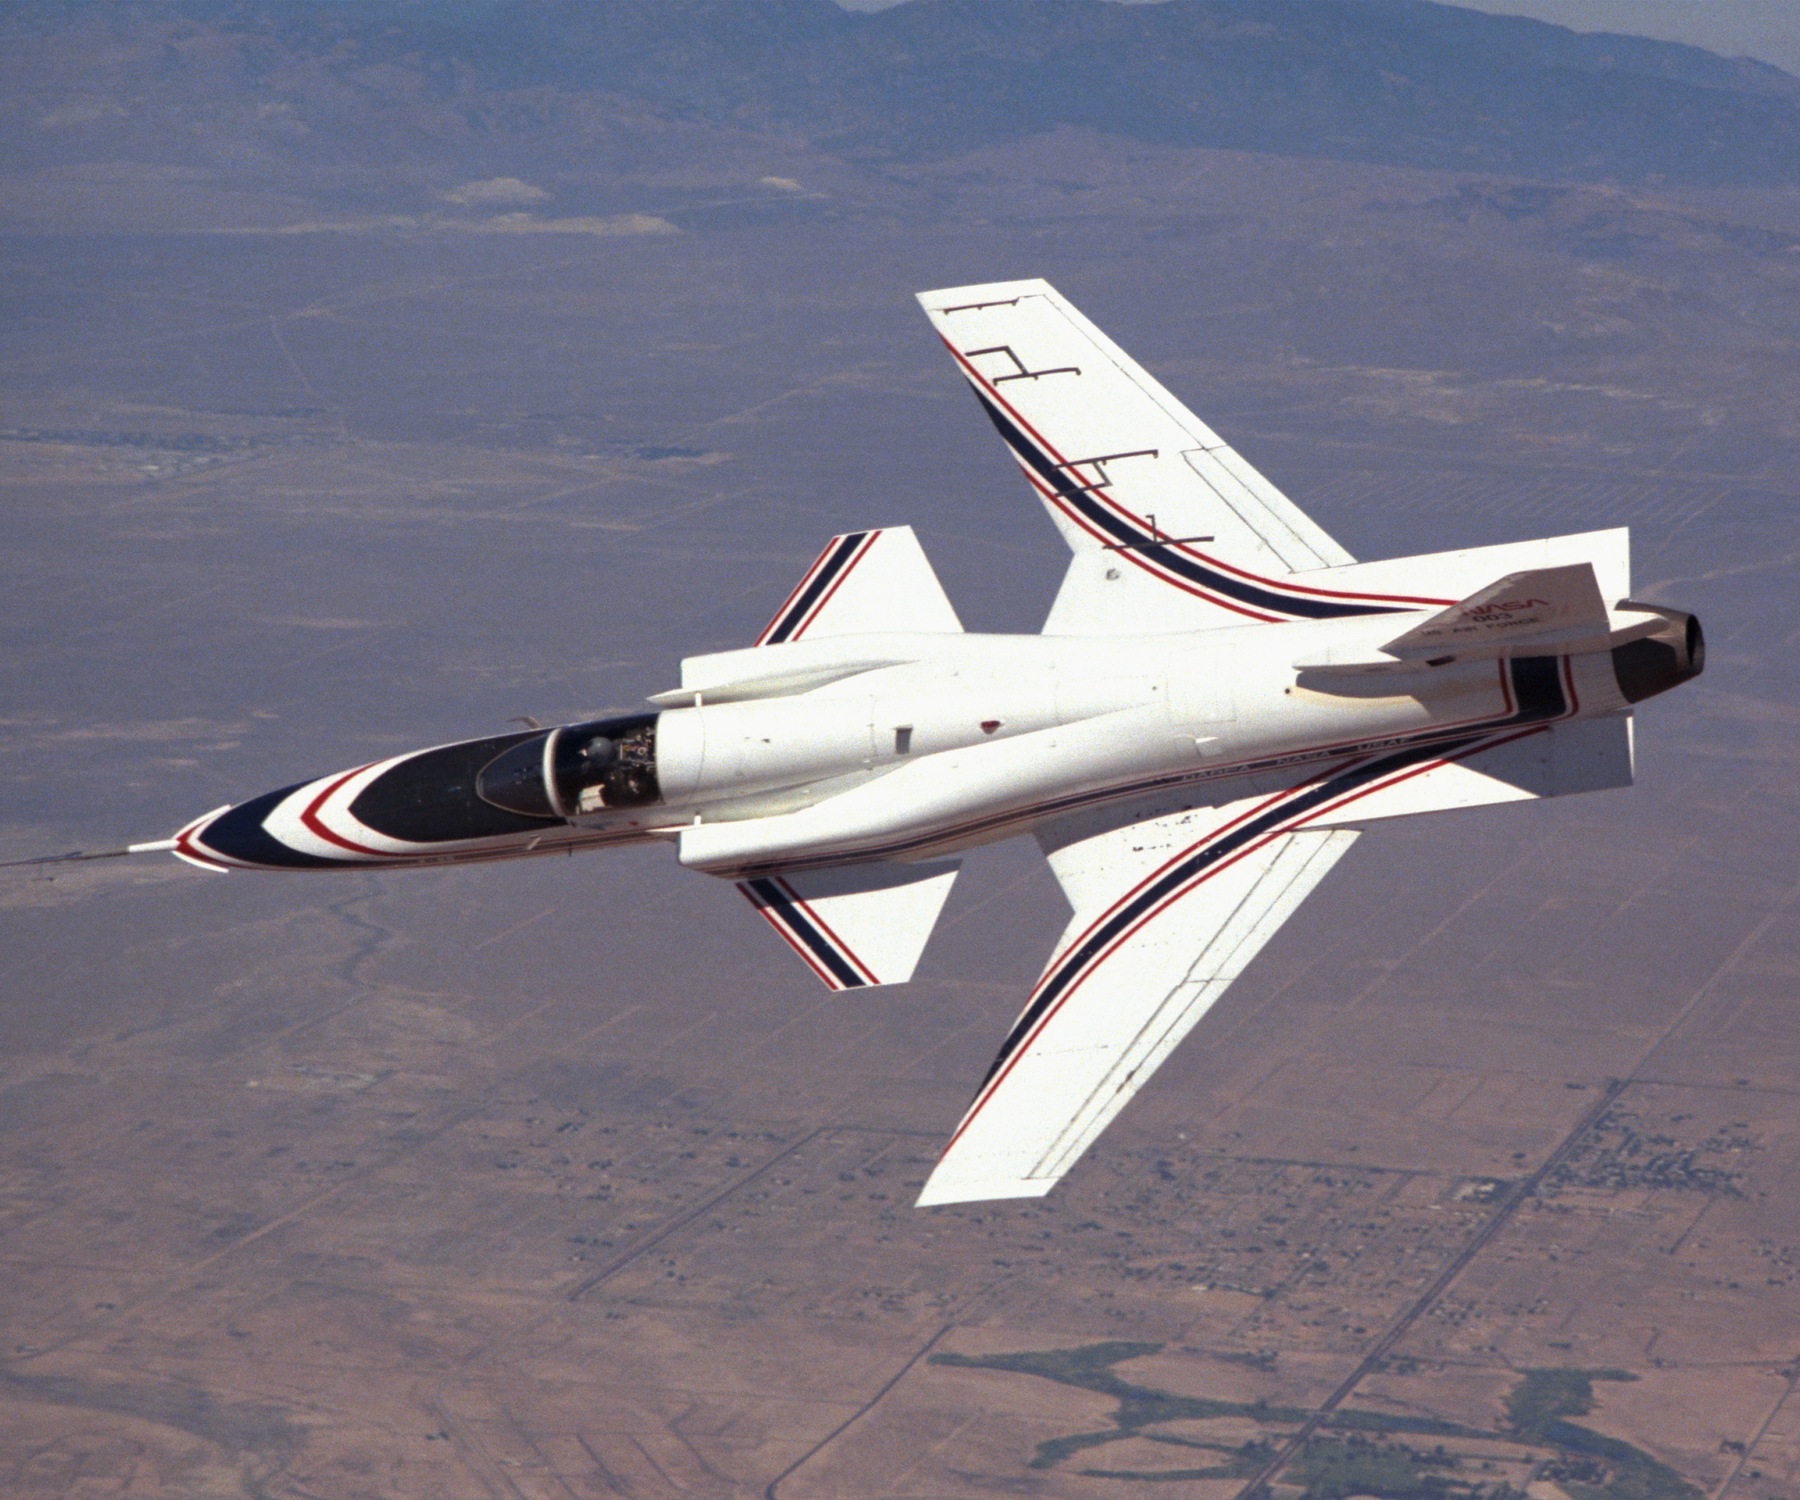
\includegraphics[width=595.276bp,height=496bp]{assets/cover-hero.jpg}};
\fill[studiumInk] (0,585.5) rectangle (595.276,841.89);
% Cabecera editorial.
% Logotipo auténtico de Studium: símbolo y letras extraídos sin redibujarlos
% de framework/docs/assets/studium-logo-dark.png, adaptados a una firma horizontal.
\node[anchor=north west,inner sep=0pt,outer sep=0pt] at (43,5)
  {
\includegraphics[width=185bp]{assets/studium-horizontal.png}};
\fill[studiumCyan] (106,76) rectangle (132,78);
\node[anchor=west,text=studiumInk,font=\sffamily\fontsize{8.2}{10}\selectfont,inner sep=0pt] at (140,79){BIBLIOTECA DE INGENIERÍA};
% Bloque inferior: tipografia, blancos y posiciones de la coleccion.
\node[anchor=west,text=studiumCyan,font=\sffamily\bfseries\fontsize{10}{12}\selectfont,inner sep=0pt] at (51.223,608){#1};
\node[anchor=north west,text=white,text width=493pt,font=\rmfamily\bfseries\fontsize{26.5}{29.5}\selectfont,inner sep=0pt] at (51.223,627){#2};
\node[anchor=north west,text=white!82!studiumInk,text width=493pt,font=\sffamily\fontsize{10}{13}\selectfont,inner sep=0pt] at (51.223,730){#3};
\node[anchor=west,text=white,font=\sffamily\bfseries\fontsize{10}{12}\selectfont,inner sep=0pt] at (51.223,774){GRADO EN INGENIERÍA AEROESPACIAL};
\node[anchor=west,text=white!82!studiumInk,font=\sffamily\fontsize{10}{12}\selectfont,inner sep=0pt] at (51.223,789){Universidad de León};
\draw[white!75!studiumInk,line width=.4pt] (51.223,801) -- (544.05,801);
\node[anchor=west,text=white!82!studiumInk,font=\sffamily\fontsize{10}{12}\selectfont,inner sep=0pt] at (51.223,822){2026};
\node[anchor=east,text=white,font=\sffamily\bfseries\fontsize{10}{12}\selectfont,inner sep=0pt] at (544.05,822){Primera edición};
\end{scope}\end{tikzpicture}\null
\end{titlepage}\hypersetup{pageanchor=true}}

\newcommand{\caso}[2]{\begin{studiumworked}{#1}#2\end{studiumworked}}
\newcommand{\ilustra}[2]{\begin{figure}[htbp]\centering\includegraphics[width=.94\linewidth]{#1.pdf}\caption{#2}\label{fig:#1}\end{figure}}
\newcommand{\fuentes}[1]{\par\medskip\noindent{\footnotesize\textbf{Fuentes y localizadores.} #1}\par}
\newcommand{\apartado}[2]{\par\medskip\noindent\textbf{#1.} #2\par}
\newcommand{\repaso}[2]{\par\medskip\noindent\textbf{Para comprobar la comprensión.} #1\par\noindent\textit{Respuesta razonada.} #2\par}

\newcommand{\vect}[1]{\boldsymbol{#1}}
\newcommand{\dd}{\mathrm{d}}
\newcommand{\SIu}[1]{\,\mathrm{#1}}
\newcommand{\hipotesis}[1]{\caja{Hipótesis y dominio}{#1}}
\newcommand{\verifica}[1]{\consejo{Comprobación y límites}{#1}}
\newcommand{\errorcomun}[1]{\caja{Error que cambia el resultado}{#1}}

\renewcommand{\studiumcoverphoto}{assets/cover-simulacros.jpg}
\hypersetup{pdftitle={Simulacros de Mecánica de Vuelo},pdfauthor={Studium}}
\begin{document}
\portada{SIMULACROS Y SOLUCIONES}{SIMULACROS\\DE MECÁNICA DE VUELO}{Seis exámenes originales · Soluciones separadas y razonadas}
\frontmatter
\chapter*{Instrucciones y constantes}
Los seis simulacros combinan competencias de ejes, actuaciones, operaciones, estabilidad y simulación. Sus datos y enunciados son originales. No son exámenes oficiales ni pronostican una convocatoria. Los problemas de dinámica del quinto simulacro están marcados como ampliación.

Use $g_0=9.80665\SIu{m/s^2}$, $R_a=287.05287\SIu{J/(kg\,K)}$, $T_0=288.15\SIu K$, $p_0=101325\SIu{Pa}$ y $\rho_0=1.225\SIu{kg/m^3}$. Hasta 11 km geopotenciales, $T=T_0-0.0065h$, $p=p_0(T/T_0)^{g_0/(0.0065R_a)}$ y $\rho=p/(R_aT)$. Los ángulos numéricos se convierten a radianes antes de evaluarse.

Se permite calculadora o un entorno numérico para las integrales y matrices; esta condición es propia del cuaderno y no una norma de evaluación ULE. Las soluciones están agrupadas después de todos los enunciados. Antes de consultarlas, explicite ley de vuelo, masa de enlace y restricciones. La revisión experta independiente continúa pendiente.
\consejo{Criterio orientativo de corrección}{Se valora el planteamiento físico y sistema de referencia, el desarrollo coherente con las hipótesis, la sustitución y las unidades, y la interpretación de restricciones. Un resultado sin modelo no equivale a una solución completa. Los repartos de puntos son docentes y no reproducen rúbricas oficiales.}
\par\smallskip
\noindent\textbf{Imagen de portada.} Fotografía NASA,
X-29 número 1 en viraje sobre el desierto de Mojave, 24 de julio de 1987., ID EC87-0182-14. Fuente: \href{https://commons.wikimedia.org/wiki/File:X-29_in_Banked_Flight.jpg}{Wikimedia Commons}.
Dominio público en Estados Unidos (autoría NASA); reutilización educativa conforme a \href{https://www.nasa.gov/nasa-brand-center/images-and-media/}{las condiciones NASA}. Recorte proporcional y remuestreo a 1800 por 1500 píxeles; sin alteración del contenido. Consulta: 19 de octubre de 2026. No implica respaldo institucional.

\tableofcontents
\mainmatter
\part{Enunciados originales}

\chapter{Ejes, planeo y maniobra}

Tiempo orientativo: 120 minutos. Puntuación total orientativa: 10 puntos. No es un examen oficial.

\section{Problema 1 · 3 puntos}

Un avión tiene Euler $(\phi,\theta,\psi)=(12,6,25)^\circ$ y velocidad aérea NED $(82,-4,-3)\SIu{m/s}$. Calcule velocidad cuerpo, TAS e incidencia. Explique por qué ascenso terrestre no determina el signo de w cuerpo.

\apartado{Datos y condiciones}{Secuencia pasiva 3--2--1; viento nulo en este caso. Horizonte local fijo, convención del manual y velocidad no nula.}

\section{Problema 2 · 4 puntos}

Un planeador de 490 kg y S=17.6 m² desciende de 3400 a 600 m ISA manteniendo CL de mejor planeo en calma. Polar 0.0132+0.0305CL². Calcule CL, alcance aéreo, duración y alcance terrestre con viento de cara 6 m/s.

\apartado{Datos y condiciones}{ISA troposférica con constantes generales del cuaderno; CLmax=1.6. Masa y polar constantes; equilibrio local exacto y sucesión cuasiestacionaria; viento vertical nulo.}

\section{Problema 3 · 3 puntos}

Una aeronave vuela a 84 m/s con alabeo 38 grados. Masa 3100 kg, S=27 m², rho=0.96 kg/m³ y CLmax=1.55. Calcule n, radio, razón de giro y CL requerido; indique qué falta para probar viraje sostenido.

\apartado{Datos y condiciones}{Viraje coordinado en calma, altitud y rapidez constantes. Empuje paralelo a velocidad; se comprueba sólo geometría y sustentación, sin mapa de propulsión.}

\chapter{Crucero de reactor y leyes de pilotaje}

Tiempo orientativo: 150 minutos. Puntuación total orientativa: 10 puntos. No es un examen oficial.

\section{Problema 1 · 4 puntos}

Un reactor de 11400 kg y masa seca 9300 kg vuela 45 minutos a 6500 m ISA con CL de máxima autonomía. S=52 m², polar 0.024+0.044CL² y cT=1.68e-5 kg/(N s). Calcule masa final, distancia y velocidades extremas.

\apartado{Datos y condiciones}{Se conservan altitud y CL; no hay viento ni reserva en este cálculo. Polar y consumo constantes; T=D; masa variable y vuelo cuasiestacionario.}

\section{Problema 2 · 4 puntos}

Desde la masa final anterior, el reactor pasa a TAS 175 m/s a la misma altitud y continúa hasta masa seca 9300 kg. Calcule duración y alcance adicionales. No mantenga artificialmente constante CL.

\apartado{Datos y condiciones}{La fase comienza en la masa de enlace calculada; polar, S, cT y altitud de la primera fase. Cambio idealizado instantáneo de velocidad sin combustible de transición; se declara como simplificación.}

\section{Problema 3 · 2 puntos}

Con los mismos datos, compruebe al inicio de la fase a TAS fija si CLmax=1.5 y empuje disponible 10500 N permiten sostener esa condición. Explique qué otra información se necesitaría.

\apartado{Datos y condiciones}{Use masa final de fase A, TAS 175 m/s y densidad ISA a 6500 m. Empuje disponible dado en ese punto; sin margen añadido ni resistencia de coordinación.}

\chapter{Hélice, potencia y combustible de misión}

Tiempo orientativo: 135 minutos. Puntuación total orientativa: 10 puntos. No es un examen oficial.

\section{Problema 1 · 3 puntos}

Un avión parte con 2180 kg, de los que 420 kg son combustible. Mantiene potencia al eje 230 kW durante siete minutos, consumo 0.30 kg/kWh y eficiencia 0.78. Calcule gasto, combustible consumido y masa al comenzar crucero.

\apartado{Datos y condiciones}{No hay otra pérdida de masa; el resto de datos se usará en el siguiente problema. Potencia y consumo específicos constantes en esa fase; no se calcula aquí la altura.}

\section{Problema 2 · 4 puntos}

Desde esa masa de enlace, el avión vuela a 2200 m ISA con CL de máximo alcance. S=21.4 m² y polar 0.028+0.049CL². Debe conservar 60 kg de combustible. Calcule masa final, alcance y tiempo, con eficiencia y consumo anteriores.

\apartado{Datos y condiciones}{Masa seca 1760 kg; reserva 60 kg: masa final requerida 1820 kg. CL, altitud, eficiencia y consumo constantes en crucero; sin viento.}

\section{Problema 3 · 3 puntos}

En una condición distinta, rho=1.02 kg/m³, m=2100 kg y TAS=59 m/s, calcule potencia necesaria con la polar anterior y tasa de ascenso aproximada con potencia al eje 230 kW. Explique por qué no basta con usar empuje máximo por un coeficiente.

\apartado{Datos y condiciones}{Eficiencia 0.78; S=21.4 m²; L≈W y polar de crucero como modelo docente. Ángulo pequeño, velocidad constante y potencia disponible en el punto.}

\chapter{Operaciones y margen estático}

Tiempo orientativo: 120 minutos. Puntuación total orientativa: 10 puntos. No es un examen oficial.

\section{Problema 1 · 4 puntos}

Un avión de 1720 kg debe alcanzar TAS 37 m/s con viento de cara 5 m/s. S=20 m², rho=1.17 kg/m³, empuje 5500 N, rodadura 0.03 y CL de carrera 0.60; polar 0.033+0.050CL². Calcule velocidad terrestre final y carrera por integración.

\apartado{Datos y condiciones}{Vaire=Vsuelo+5 m/s; pista horizontal. Empuje finito constante; coeficientes de carrera fijos y reacción no negativa.}

\section{Problema 2 · 3 puntos}

En calma, la misma aeronave toma a 29 m/s con CL residual 0.16, freno 0.29 y empuje nulo. Calcule carrera de frenado y distancia añadida por una demora de 1.2 s a velocidad media prescrita de 28 m/s.

\apartado{Datos y condiciones}{S, densidad y polar anteriores; la demora es una fase adicional. Frenado de Coulomb, coeficientes constantes, sin pendiente ni empuje inverso.}

\section{Problema 3 · 3 puntos}

Un modelo tiene aw=5.1, at=4.2, St/S=0.18, $eta_{t}$=0.9, $epsilon_{alpha}$=0.35, hac=0.25, ht=3.1 y $Cm_{alpha,f}$=0.06. Calcule hn, margen para h=0.35 y $Cm_{alpha}$. ¿Prueba esto estabilidad dinámica?

\apartado{Datos y condiciones}{Pendientes por radián, posiciones hacia atrás en unidades de cuerda. Mando fijo y aerodinámica lineal; mismo datum y configuración.}

\chapter{Newton--Euler y estabilidad como ampliación}

Tiempo orientativo: 135 minutos. Puntuación total orientativa: 10 puntos. No es un examen oficial.

\section{Problema 1 · 4 puntos}

Use Ixx=11000, Iyy=16500, Izz=21000 e Ixz=850 kg m², con entradas cruzadas negativas. Para omega=(0.10,0.06,-0.08) rad/s y momentos (700,-450,380) N m, calcule aceleraciones y compruebe el balance vectorial.

\apartado{Datos y condiciones}{Tensor constante y momentos respecto al CG. Sólido rígido simétrico, sin masa móvil ni flujo de momento angular.}

\section{Problema 2 · 3 puntos}

Para q=2400 Pa, Sv=4.5 m², eficiencia 0.93, av=3.9/rad, $x_{v}$=-5.8 m y beta=2.5 grados, calcule fuerza y momento de cola. Razone el signo de $Cn_{beta}$ y qué dato faltaría para amortiguamiento en guiñada.

\apartado{Datos y condiciones}{Flujo local beta igual al global; cola detrás del CG. Cola lineal y sin interferencia; no hay timón.}

\section{Problema 3 · 3 puntos}

Como ampliación, estudie una ecuación sintética xddot+0.5 xdot+3.24x=0. Calcule autovalores, periodo y tiempo de reducción a la mitad. Compare con cambiar el signo del término de tasa.

\apartado{Datos y condiciones}{x adimensional, tiempo en segundos; no es modelo de una aeronave identificada. Sistema lineal autónomo sin forzamiento.}

\chapter{Auditoría de simulación y decisión de modelo}

Tiempo orientativo: 120 minutos. Puntuación total orientativa: 10 puntos. No es un examen oficial.

\section{Problema 1 · 4 puntos}

En el experimento original B747 de 28000 lbm, el tiempo simulado hasta agotamiento es el de los datos adjuntos. Compare con congelar el gasto inicial y con el modelo equivalente. Calcule diferencias relativas y explique por qué ninguna constituye validación experimental.

\apartado{Datos y condiciones}{Tiempo simulado 4113.000000 s; gasto constante 4003.098950 s; equivalente 4105.333000 s. Deriva máxima de altura 58.253 m; paso 0.1 s. Datos realmente ejecutados del modelo educativo, no mediciones de avión real.}

\section{Problema 2 · 3 puntos}

Un registro sintético indica empuje máximo 2500 lbf, factor de tabla 0.64, TAS 340 ft/s y EAS 285 ft/s. Calcule empuje disponible, potencia correcta y error al multiplicar por EAS. Identifique el error dimensional de llamar potencia al empuje por el factor.

\apartado{Datos y condiciones}{1 lbf=4.448221615 N y 1 ft=0.3048 m; datos sintéticos originales. Factor adimensional de empuje y velocidad alineada con empuje.}

\section{Problema 3 · 3 puntos}

Dos configuraciones docentes tienen la misma sustentación requerida CL=0.85. Limpia: CD0=0.025, k=0.045. Flaps: CD0=0.040, k=0.047. Con qS=29000 N y empuje 4400 N, calcule márgenes de empuje. ¿Permite concluir qué configuración tiene mayor ángulo máximo global?

\apartado{Datos y condiciones}{Comparación a la misma condición local y mismo empuje; no son datos SAULE. Polar parabólica, mismas referencias y L=qS CL; empuje paralelo a trayectoria.}

\part{Soluciones desarrolladas}

\chapter{Soluciones: Ejes, planeo y maniobra}



\section{Problema 1: Reconstrucción de velocidad y actitud}

\apartado{2. Datos}{Secuencia pasiva 3--2--1; viento nulo en este caso.}

\apartado{3. Incógnitas}{Magnitudes y conclusiones solicitadas en el enunciado.}

\apartado{4. Sistema de referencia}{Cuerpo x adelante, y derecha, z abajo; NED cuando corresponda.}

\apartado{5. Hipótesis físicas}{Horizonte local fijo, convención del manual y velocidad no nula.}

\apartado{6. Modelo matemático}{Reconstrucción de velocidad y actitud}

\apartado{7. Ecuaciones simbólicas}{Se parte de los balances y definiciones siguientes.}

\begin{equation}\vect v_a^b=C_{bn}\vect v_a^n\end{equation}

\begin{equation}V=\|\vect v_a\|,\quad\alpha=\operatorname{atan2}(w_a,u_a)\end{equation}

\apartado{8. Desarrollo algebraico}{Las operaciones se realizan en este orden, conservando las condiciones del modelo.}

\begin{enumerate}

\item Se construyen las tres rotaciones en orden y se multiplican por la velocidad NED.

\item Se calcula la norma y se compara antes y después de rotar.

\item El vector NED tiene componente abajo negativa, pero el componente cuerpo incluye la actitud.

\end{enumerate}

\apartado{9. Sustitución numérica}{Se conservan los resultados intermedios sin redondear y se muestran todas las operaciones escalares disponibles.}

\textbf{Construcción de la matriz y producto por filas.} Se convierte cada ángulo a radianes y se escribe $c_\phi=\cos\phi$, $s_\phi=\sin\phi$, y análogamente para los otros ángulos. Multiplicar las rotaciones pasivas en orden 3--2--1 da:\[\fitmath{C_{bn}=\begin{bmatrix}c_\theta c_\psi&c_\theta s_\psi&-s_\theta\\s_\phi s_\theta c_\psi-c_\phi s_\psi&s_\phi s_\theta s_\psi+c_\phi c_\psi&s_\phi c_\theta\\c_\phi s_\theta c_\psi+s_\phi s_\psi&c_\phi s_\theta s_\psi-s_\phi c_\psi&c_\phi c_\theta\end{bmatrix}}\]\[\fitmath{u=(0.901342938)(82)+(0.420303115)(-4)+(-0.104528463)(-3)\approx72.54249\,\mathrm{m/s}}\]\[\fitmath{v=(-0.393686533)(82)+(0.895687419)(-4)+(0.206772729)(-3)\approx-36.48536\,\mathrm{m/s}}\]\[\fitmath{w=(0.180532051)(82)+(-0.145221691)(-4)+(0.972789206)(-3)\approx12.46615\,\mathrm{m/s}}\]La inversa es la transpuesta: multiplicar $C_{bn}^T$ por el vector obtenido recupera las tres componentes NED. Las normas coinciden: $V=82.1523\,\mathrm{m/s}$. Para incidencia se usa $\alpha=\operatorname{atan2}(w,u)$; el argumento de $w/u$ por sí solo pierde el cuadrante.


\begin{enumerate}

\item TAS.

\[\fitmath{y_{4}=\sqrt{{82}^{2}+{4}^{2}+{3}^{2}}\approx 82.1523\,\mathrm{m/s}}\]

\end{enumerate}


\apartado{10. Resultados con unidades}{Los resultados pertenecen al modelo y al intervalo de datos declarados.}

\begin{center}\begin{tabular}{lr}\toprule Magnitud&Resultado\\\midrule

u cuerpo & $72.54249\,\mathrm{m\,s^{-1}}$\\

v cuerpo & $-36.48536\,\mathrm{m\,s^{-1}}$\\

w cuerpo & $12.46615\,\mathrm{m\,s^{-1}}$\\

TAS & $82.1523\,\mathrm{m\,s^{-1}}$\\

Incidencia & $0.1701839\,\mathrm{rad}$\\

\bottomrule\end{tabular}\end{center}

\apartado{11. Interpretación}{El ascenso se reconoce en NED; incidencia y w describen la dirección relativa al fuselaje.}

\apartado{12. Comprobación independiente y alcance}{Aplicar la transpuesta para recuperar el vector NED y comprobar norma y determinante.}

\apartado{13. Limitaciones}{El replay de los tres componentes literales no prueba la multiplicación: se conserva la prueba matricial de ida y vuelta.}

\par\smallskip\noindent{\footnotesize\textit{Datos y solución originales. Las sustituciones registradas se reproducen con SymPy y Studium; eso no establece validación experimental ni revisión experta.}}


\section{Problema 2: Alcance y duración con atmósfera variable}

\apartado{2. Datos}{ISA troposférica con constantes generales del cuaderno; CLmax=1.6.}

\apartado{3. Incógnitas}{Magnitudes y conclusiones solicitadas en el enunciado.}

\apartado{4. Sistema de referencia}{Trayectoria aérea descendente, gamma<0; ruta terrestre alineada con viento.}

\apartado{5. Hipótesis físicas}{Masa y polar constantes; equilibrio local exacto y sucesión cuasiestacionaria; viento vertical nulo.}

\apartado{6. Modelo matemático}{Alcance y duración con atmósfera variable}

\apartado{7. Ecuaciones simbólicas}{Se parte de los balances y definiciones siguientes.}

\begin{equation}C_L=\sqrt{C_{D0}/k},\quad\delta=\arctan(C_D/C_L)\end{equation}

\begin{equation}R_a=\Delta hC_L/C_D\end{equation}

\begin{equation}E=\int_{h_f}^{h_i}\dd h/s(h),\quad R_g=R_a-6E\end{equation}

\apartado{8. Desarrollo algebraico}{Las operaciones se realizan en este orden, conservando las condiciones del modelo.}

\begin{enumerate}

\item Se obtiene CL y se comprueba con CLmax.

\item Se usa ángulo exacto para la velocidad local y descenso.

\item Se integra con densidad ISA y se resta el desplazamiento de viento durante todo el tiempo.

\end{enumerate}

\apartado{9. Sustitución numérica}{Se conservan los resultados intermedios sin redondear y se muestran todas las operaciones escalares disponibles.}

\textbf{Integral de tiempo desarrollada.} Calcular $C_D=C_{D0}+kC_L^2$ y $\delta=\arctan(C_D/C_L)$. Del equilibrio exacto, $V(h)=\sqrt{2mg_0\cos\delta/[\rho(h)SC_L]}$ y $s(h)=V(h)\sin\delta$. Definir $K=\sqrt{2mg_0\cos\delta/(SC_L)}\sin\delta$ da $s=K/\sqrt\rho$. En la troposfera, $\rho=\rho_0(1-\beta h/T_0)^a$, con $a=g_0/(R\beta)-1$.\[\fitmath{E=\frac{\sqrt{\rho_0}}{K}\int_{h_f}^{h_i}(1-\beta h/T_0)^{a/2}dh=\frac{\sqrt{\rho_0}T_0}{K\beta(1+a/2)}\left[(1-\beta h_f/T_0)^{1+a/2}-(1-\beta h_i/T_0)^{1+a/2}\right]}\]Los parámetros intermedios son $C_L=0.6578654$, $C_D=0.0264$, $\delta=0.04010827\,\mathrm{rad}$ y $a=4.25588$. La evaluación por alturas permite contrastar el integrando:\begin{center}\begin{tabular}{rrrrr}
\toprule $h$ (m) & $
ho$ & $V$ (m/s) & $s$ (m/s) & $1/s$ (s/m)\\\midrule
$600$ & $1.155977$ & $26.78547$ & $1.074031$ & $0.9310721$\\
$1300$ & $1.079255$ & $27.72119$ & $1.111551$ & $0.899644$\\
$2000$ & $1.00649$ & $28.70576$ & $1.15103$ & $0.8687873$\\
$2700$ & $0.9375395$ & $29.74261$ & $1.192605$ & $0.8385009$\\
$3400$ & $0.8722622$ & $30.83545$ & $1.236425$ & $0.8087834$\\
\bottomrule\end{tabular}\end{center}\[\fitmath{E\approx2433.669\,\mathrm s,\qquad R_a=(h_i-h_f)\frac{C_L}{C_D}\approx69773.6\,\mathrm m}\]\[\fitmath{R_g=R_a+U E\approx55171.59\,\mathrm m}\]


\begin{enumerate}

\item CL óptimo.

\[\fitmath{y_{1}=\sqrt{\frac{0.0132}{0.0305}}\approx 0.6578654\,}\]

\end{enumerate}


\apartado{10. Resultados con unidades}{Los resultados pertenecen al modelo y al intervalo de datos declarados.}

\begin{center}\begin{tabular}{lr}\toprule Magnitud&Resultado\\\midrule

CL óptimo & $0.6578654\,$\\

Alcance aéreo & $69773.6\,\mathrm m$\\

Duración & $2433.669\,\mathrm s$\\

Alcance terrestre & $55171.59\,\mathrm m$\\

\bottomrule\end{tabular}\end{center}

\apartado{11. Interpretación}{No se reoptimiza el vuelo para viento; se evalúa la ley explícitamente impuesta.}

\apartado{12. Comprobación independiente y alcance}{Comparar cuadratura con la primitiva de potencia de temperatura y comprobar que Ra/E no se confunde con la TAS inicial.}

\apartado{13. Limitaciones}{La variación lenta de TAS se omite en el balance inercial local.}

\par\smallskip\noindent{\footnotesize\textit{Datos y solución originales. Las sustituciones registradas se reproducen con SymPy y Studium; eso no establece validación experimental ni revisión experta.}}


\section{Problema 3: Viraje nivelado y pérdida}

\apartado{2. Datos}{Viraje coordinado en calma, altitud y rapidez constantes.}

\apartado{3. Incógnitas}{Magnitudes y conclusiones solicitadas en el enunciado.}

\apartado{4. Sistema de referencia}{Cuerpo x adelante, y derecha, z abajo; NED cuando corresponda.}

\apartado{5. Hipótesis físicas}{Empuje paralelo a velocidad; se comprueba sólo geometría y sustentación, sin mapa de propulsión.}

\apartado{6. Modelo matemático}{Viraje nivelado y pérdida}

\apartado{7. Ecuaciones simbólicas}{Se parte de los balances y definiciones siguientes.}

\begin{equation}n=1/\cos\phi,\quad R=V^2/(g_0\tan\phi)\end{equation}

\begin{equation}\dot\chi=g_0\tan\phi/V,\quad C_L=2nmg_0/(\rho V^2S)\end{equation}

\apartado{8. Desarrollo algebraico}{Las operaciones se realizan en este orden, conservando las condiciones del modelo.}

\begin{enumerate}

\item La sustentación se incrementa a nW.

\item Se calcula la aceleración centrípeta y se obtiene el radio.

\item Se verifica CL y se identifica que falta resistencia y empuje disponible para sostenibilidad.

\end{enumerate}

\apartado{9. Sustitución numérica}{Se conservan los resultados intermedios sin redondear y se muestran todas las operaciones escalares disponibles.}

\begin{enumerate}

\item n.

\[\fitmath{y_{1}=\frac{1}{\cos\left(\frac{38\cdot \pi}{180}\right)}\approx 1.269018\,}\]

\item Radio.

\[\fitmath{y_{2}=\frac{{84}^{2}}{9.80665\cdot \tan\left(\frac{38\cdot \pi}{180}\right)}\approx 920.9331\,\mathrm{m}}\]

\item Razón.

\[\fitmath{y_{3}=\frac{9.80665\cdot \tan\left(\frac{38\cdot \pi}{180}\right)}{84}\approx 0.09121184\,\mathrm{1/s}}\]

\item CL requerido.

\[\fitmath{y_{4}=\frac{2\cdot 3100\cdot 9.80665}{\cos\left(\frac{38\cdot \pi}{180}\right)\cdot 0.96\cdot {84}^{2}\cdot 27}\approx 0.4218778\,}\]

\end{enumerate}


\apartado{10. Resultados con unidades}{Los resultados pertenecen al modelo y al intervalo de datos declarados.}

\begin{center}\begin{tabular}{lr}\toprule Magnitud&Resultado\\\midrule

n & $1.269018\,$\\

Radio & $920.9331\,\mathrm m$\\

Razón & $0.09121184\,\mathrm{s^{-1}}$\\

CL requerido & $0.4218778\,$\\

\bottomrule\end{tabular}\end{center}

\apartado{11. Interpretación}{La geometría puede ser posible por sustentación y aun no ser sostenible por motor.}

\apartado{12. Comprobación independiente y alcance}{Comprobar n g sin(phi)=V²/R y CL<=CLmax.}

\apartado{13. Limitaciones}{Sin límite estructural ni trim de momentos.}

\par\smallskip\noindent{\footnotesize\textit{Datos y solución originales. Las sustituciones registradas se reproducen con SymPy y Studium; eso no establece validación experimental ni revisión experta.}}




\chapter{Soluciones: Crucero de reactor y leyes de pilotaje}



\section{Problema 1: Primera fase de autonomía}

\apartado{2. Datos}{Se conservan altitud y CL; no hay viento ni reserva en este cálculo.}

\apartado{3. Incógnitas}{Magnitudes y conclusiones solicitadas en el enunciado.}

\apartado{4. Sistema de referencia}{Ruta horizontal y ejes viento; TAS variable.}

\apartado{5. Hipótesis físicas}{Polar y consumo constantes; T=D; masa variable y vuelo cuasiestacionario.}

\apartado{6. Modelo matemático}{Primera fase de autonomía}

\apartado{7. Ecuaciones simbólicas}{Se parte de los balances y definiciones siguientes.}

\begin{equation}C_L=\sqrt{C_{D0}/k}\end{equation}

\begin{equation}m_f=m_i\exp[-g_0c_Tt/(C_L/C_D)]\end{equation}

\begin{equation}R=K_m(\sqrt{m_i}-\sqrt{m_f})\end{equation}

\apartado{8. Desarrollo algebraico}{Las operaciones se realizan en este orden, conservando las condiciones del modelo.}

\begin{enumerate}

\item Se utiliza CL de autonomía de reactor.

\item Se invierte la integral temporal logarítmica para encontrar masa.

\item Se integra la velocidad variable para alcance y se calculan ambos extremos de TAS.

\end{enumerate}

\apartado{9. Sustitución numérica}{Se conservan los resultados intermedios sin redondear y se muestran todas las operaciones escalares disponibles.}

\textbf{Desarrollo de las magnitudes intermedias.} De $dm/dt=-c_TD=-c_Tmg_0/(L/D)$, separar variables da $E=(L/D)\ln(m_i/m_f)/(g_0c_T)$. Con CL fijo, $V=\sqrt{2g_0m/(\rho SC_L)}$; sustituir en $dx=Vdt$ deja integrar $m^{-1/2}$, cuya primitiva es $2\sqrt m$. Por eso $R=K_m(\sqrt{m_i}-\sqrt{m_f})$, con $K_m=2(L/D)\sqrt{2g_0/(\rho SC_L)}/(g_0c_T)$. Aquí se fija duración y se invierte la integral de tiempo: $m_f=m_i\exp[-g_0c_TE/(L/D)]$. Para autonomía de reactor se maximiza $L/D$ y se usa $C_L=\sqrt{C_{D0}/k}$.\begin{enumerate}

\item Óptimo de autonomía del reactor.

\[\fitmath{C_L=\sqrt{\frac{0.024}{0.044}}\approx 0.7385489\,}\]

\item Eficiencia correspondiente.

\[\fitmath{\mathrm{LD}=\frac{C_L}{0.024+0.044\cdot {C_L}^{2}}}\]

\[\fitmath{\mathrm{LD}=\frac{(0.7385489459)}{0.024+0.044\cdot {(0.7385489459)}^{2}}\approx 15.38644\,}\]

\item Invertir el logaritmo de la ley temporal.

\[\fitmath{\mathrm{mf}=11400\cdot \exp\left(\frac{-9.80665\cdot 1.68\times10^{-5}\cdot 2700}{\mathrm{LD}}\right)}\]

\[\fitmath{\mathrm{mf}=11400\cdot \exp\left(\frac{-9.80665\cdot 1.68\times10^{-5}\cdot 2700}{(15.38643637)}\right)\approx 11075.14\,\mathrm{kg}}\]

\item Evaluar el coeficiente de distancia.

\[\fitmath{\mathrm{Km}=\frac{2\cdot \mathrm{LD}}{9.80665\cdot 1.68\times10^{-5}}\cdot \sqrt{\frac{2\cdot 9.80665}{0.623843718\cdot 52\cdot C_L}}}\]

\[\fitmath{\mathrm{Km}=\frac{2\cdot (15.38643637)}{9.80665\cdot 1.68\times10^{-5}}\cdot \sqrt{\frac{2\cdot 9.80665}{0.623843718\cdot 52\cdot (0.7385489459)}}\approx 168999\,\mathrm{m/kg^{.5}}}\]

\item Integrar la velocidad que disminuye con la masa.

\[\fitmath{R=\mathrm{Km}\cdot \left(\sqrt{11400}-\sqrt{\mathrm{mf}}\right)}\]

\[\fitmath{R=(168999.0265)\cdot \left(\sqrt{11400}-\sqrt{(11075.13882)}\right)\approx 258956.7\,\mathrm{m}}\]

\item Velocidad inicial.

\[\fitmath{\mathrm{Vi}=\sqrt{\frac{2\cdot 11400\cdot 9.80665}{0.623843718\cdot 52\cdot C_L}}}\]

\[\fitmath{\mathrm{Vi}=\sqrt{\frac{2\cdot 11400\cdot 9.80665}{0.623843718\cdot 52\cdot (0.7385489459)}}\approx 96.60476\,\mathrm{m/s}}\]

\item Velocidad final.

\[\fitmath{\mathrm{Vf}=\sqrt{\frac{2\cdot \mathrm{mf}\cdot 9.80665}{0.623843718\cdot 52\cdot C_L}}}\]

\[\fitmath{\mathrm{Vf}=\sqrt{\frac{2\cdot (11075.13882)\cdot 9.80665}{0.623843718\cdot 52\cdot (0.7385489459)}}\approx 95.21836\,\mathrm{m/s}}\]

\end{enumerate}


\begin{enumerate}

\item Masa final.

\[\fitmath{y_{1}=11400\cdot \exp\left(\frac{-9.80665\cdot 1.68\times10^{-5}\cdot 2700}{15.38643637}\right)\approx 11075.14\,\mathrm{kg}}\]

\end{enumerate}


\apartado{10. Resultados con unidades}{Los resultados pertenecen al modelo y al intervalo de datos declarados.}

\begin{center}\begin{tabular}{lr}\toprule Magnitud&Resultado\\\midrule

Masa final & $11075.14\,\mathrm{kg}$\\

Distancia & $258956.7\,\mathrm m$\\

Vi & $96.60476\,\mathrm{m\,s^{-1}}$\\

Vf & $95.21836\,\mathrm{m\,s^{-1}}$\\

\bottomrule\end{tabular}\end{center}

\apartado{11. Interpretación}{La velocidad disminuye con masa aunque la altitud no cambie.}

\apartado{12. Comprobación independiente y alcance}{Integrar dm/dt y dx/dt con la ley CL fija y comprobar mA mayor que masa seca.}

\apartado{13. Limitaciones}{Se omiten ascenso y transitorios de mando.}

\par\smallskip\noindent{\footnotesize\textit{Datos y solución originales. Las sustituciones registradas se reproducen con SymPy y Studium; eso no establece validación experimental ni revisión experta.}}


\section{Problema 2: Segunda fase a TAS fija}

\apartado{2. Datos}{La fase comienza en la masa de enlace calculada; polar, S, cT y altitud de la primera fase.}

\apartado{3. Incógnitas}{Magnitudes y conclusiones solicitadas en el enunciado.}

\apartado{4. Sistema de referencia}{Vuelo horizontal en calma; TAS constante y CL variable.}

\apartado{5. Hipótesis físicas}{Cambio idealizado instantáneo de velocidad sin combustible de transición; se declara como simplificación.}

\apartado{6. Modelo matemático}{Segunda fase a TAS fija}

\apartado{7. Ecuaciones simbólicas}{Se parte de los balances y definiciones siguientes.}

\begin{equation}D(W)=A_V+B_VW^2\end{equation}

\begin{equation}E=\frac{\arctan(W_i\sqrt{B_V/A_V})-\arctan(W_f\sqrt{B_V/A_V})}{g_0c_T\sqrt{A_VB_V}}\end{equation}

\begin{equation}R=175E\end{equation}

\apartado{8. Desarrollo algebraico}{Las operaciones se realizan en este orden, conservando las condiciones del modelo.}

\begin{enumerate}

\item Se actualiza la masa inicial de la fase.

\item Se calcula el nuevo CL para cada peso con la misma TAS.

\item Se evalúa la integral arcotangente y se añade al tiempo y distancia de la fase anterior si se solicita misión total.

\end{enumerate}

\apartado{9. Sustitución numérica}{Se conservan los resultados intermedios sin redondear y se muestran todas las operaciones escalares disponibles.}

\textbf{Desarrollo de las magnitudes intermedias.} Al cambiar a TAS fija, la resistencia pasa a $D=A+BW^2$, con $A=qSC_{D0}$ y $B=k/(qS)$. Separar la ecuación de consumo y sustituir $u=W\sqrt{B/A}$ produce la primitiva arcotangente; la masa de enlace es la calculada en la fase anterior.\begin{enumerate}

\item Término parásito a TAS fija.

\[\fitmath{A=0.5\cdot 0.623843718\cdot {175}^{2}\cdot 52\cdot 0.024\approx 11921.65\,\mathrm{N}}\]

\item Coeficiente del peso al cuadrado.

\[\fitmath{B=\frac{2\cdot 0.044}{0.623843718\cdot {175}^{2}\cdot 52}\approx 8.857832\times10^{-8}\,\mathrm{1/N}}\]

\item Evaluar la diferencia de primitivas.

\[\fitmath{E=\frac{\arctan\left(11075.13882\cdot 9.80665\cdot \sqrt{\frac{B}{A}}\right)-\arctan\left(9300\cdot 9.80665\cdot \sqrt{\frac{B}{A}}\right)}{9.80665\cdot 1.68\times10^{-5}\cdot \sqrt{A\cdot B}}}\]

\[\fitmath{E=\frac{\arctan\left(11075.13882\cdot 9.80665\cdot \sqrt{\frac{(8.857831713\times10^{-8})}{(11921.65345)}}\right)-\arctan\left(9300\cdot 9.80665\cdot \sqrt{\frac{(8.857831713\times10^{-8})}{(11921.65345)}}\right)}{9.80665\cdot 1.68\times10^{-5}\cdot \sqrt{(11921.65345)\cdot (8.857831713\times10^{-8})}}\approx 8250.161\,\mathrm{s}}\]

\item En esta fase sí es válida distancia igual a TAS constante por tiempo.

\[\fitmath{R=175\cdot E}\]

\[\fitmath{R=175\cdot (8250.160621)\approx 1443778\,\mathrm{m}}\]

\item Cerrar consumo de la segunda fase.

\[\fitmath{\mathrm{fuel}=11075.13882-9300\approx 1775.139\,\mathrm{kg}}\]

\end{enumerate}


\begin{enumerate}

\item Combustible de la segunda fase.

\[\fitmath{y_{3}=11075.13882-9300\approx 1775.139\,\mathrm{kg}}\]

\end{enumerate}


\apartado{10. Resultados con unidades}{Los resultados pertenecen al modelo y al intervalo de datos declarados.}

\begin{center}\begin{tabular}{lr}\toprule Magnitud&Resultado\\\midrule

Tiempo adicional & $8250.161\,\mathrm s$\\

Distancia adicional & $1443778\,\mathrm m$\\

Combustible de la segunda fase & $1775.139\,\mathrm{kg}$\\

\bottomrule\end{tabular}\end{center}

\apartado{11. Interpretación}{Cambiar la ley de vuelo obliga a cambiar la integral, conservando masa de enlace.}

\apartado{12. Comprobación independiente y alcance}{ODE de masa a TAS fija con evento final 9300 kg y comparación con arcotangente.}

\apartado{13. Limitaciones}{La aceleración entre leyes no se ha modelado y debe añadirse en una misión física más precisa.}

\par\smallskip\noindent{\footnotesize\textit{Datos y solución originales. Las sustituciones registradas se reproducen con SymPy y Studium; eso no establece validación experimental ni revisión experta.}}


\section{Problema 3: Comprobación de dos restricciones}

\apartado{2. Datos}{Use masa final de fase A, TAS 175 m/s y densidad ISA a 6500 m.}

\apartado{3. Incógnitas}{Magnitudes y conclusiones solicitadas en el enunciado.}

\apartado{4. Sistema de referencia}{Cuerpo x adelante, y derecha, z abajo; NED cuando corresponda.}

\apartado{5. Hipótesis físicas}{Empuje disponible dado en ese punto; sin margen añadido ni resistencia de coordinación.}

\apartado{6. Modelo matemático}{Comprobación de dos restricciones}

\apartado{7. Ecuaciones simbólicas}{Se parte de los balances y definiciones siguientes.}

\begin{equation}C_L=2mg_0/(\rho V^2S)\end{equation}

\begin{equation}D=q_\infty S(C_{D0}+kC_L^2)\end{equation}

\begin{equation}M_T=T_d-D\end{equation}

\apartado{8. Desarrollo algebraico}{Las operaciones se realizan en este orden, conservando las condiciones del modelo.}

\begin{enumerate}

\item Se calcula CL con la masa real de enlace.

\item Se evalúa resistencia y margen de empuje.

\item Ambas desigualdades son necesarias; faltan trim, Mach y otras limitaciones.

\end{enumerate}

\apartado{9. Sustitución numérica}{Se conservan los resultados intermedios sin redondear y se muestran todas las operaciones escalares disponibles.}

\textbf{Desarrollo de las magnitudes intermedias.} La factibilidad por sustentación se contrasta con $C_{L,max}$; la de motor compara la resistencia de ese mismo estado con el empuje disponible. Ninguna de las dos verifica por sí sola el trim de momentos.\begin{enumerate}

\item Fuerza de referencia de la fase a TAS fija.

\[\fitmath{\mathrm{qS}=0.5\cdot 0.623843718\cdot {175}^{2}\cdot 52\approx 496735.6\,\mathrm{N}}\]

\item Sustentación requerida por la masa de enlace.

\[\fitmath{C_L=\frac{11075.13882\cdot 9.80665}{\mathrm{qS}}}\]

\[\fitmath{C_L=\frac{11075.13882\cdot 9.80665}{(496735.5604)}\approx 0.2186475\,}\]

\item Resistencia y empuje requerido.

\[\fitmath{D=\mathrm{qS}\cdot \left(0.024+0.044\cdot {C_L}^{2}\right)}\]

\[\fitmath{D=(496735.5604)\cdot \left(0.024+0.044\cdot {(0.2186475436)}^{2}\right)\approx 12966.54\,\mathrm{N}}\]

\item Margen local de empuje disponible.

\[\fitmath{\mathrm{margin}=10500-D}\]

\[\fitmath{\mathrm{margin}=10500-(12966.53518)\approx -2466.535\,\mathrm{N}}\]

\end{enumerate}


\begin{enumerate}

\item CL de entrada.

\[\fitmath{y_{1}=\frac{2\cdot 11075.13882\cdot 9.80665}{0.623843718\cdot {175}^{2}\cdot 52}\approx 0.2186475\,}\]

\end{enumerate}


\apartado{10. Resultados con unidades}{Los resultados pertenecen al modelo y al intervalo de datos declarados.}

\begin{center}\begin{tabular}{lr}\toprule Magnitud&Resultado\\\midrule

CL de entrada & $0.2186475\,$\\

Resistencia & $12966.54\,\mathrm N$\\

Margen de empuje & $-2466.535\,\mathrm N$\\

\bottomrule\end{tabular}\end{center}

\apartado{11. Interpretación}{Un margen positivo de empuje no demuestra estabilidad ni autoridad de elevador.}

\apartado{12. Comprobación independiente y alcance}{Sustituir T=D+MT y comprobar la magnitud de cada componente de resistencia.}

\apartado{13. Limitaciones}{El empuje se da sólo para esta condición, sin mapa completo.}

\par\smallskip\noindent{\footnotesize\textit{Datos y solución originales. Las sustituciones registradas se reproducen con SymPy y Studium; eso no establece validación experimental ni revisión experta.}}




\chapter{Soluciones: Hélice, potencia y combustible de misión}



\section{Problema 1: Consumo de ascenso y masa de enlace}

\apartado{2. Datos}{No hay otra pérdida de masa; el resto de datos se usará en el siguiente problema.}

\apartado{3. Incógnitas}{Magnitudes y conclusiones solicitadas en el enunciado.}

\apartado{4. Sistema de referencia}{Cuerpo x adelante, y derecha, z abajo; NED cuando corresponda.}

\apartado{5. Hipótesis físicas}{Potencia y consumo específicos constantes en esa fase; no se calcula aquí la altura.}

\apartado{6. Modelo matemático}{Consumo de ascenso y masa de enlace}

\apartado{7. Ecuaciones simbólicas}{Se parte de los balances y definiciones siguientes.}

\begin{equation}\dot m_f=c_PP_{eje}\end{equation}

\begin{equation}m_{fin}=m_0-c_PP_{eje}t\end{equation}

\apartado{8. Desarrollo algebraico}{Las operaciones se realizan en este orden, conservando las condiciones del modelo.}

\begin{enumerate}

\item Se distingue potencia al eje de potencia de empuje.

\item Se convierte tiempo a horas o consumo a kg/J de forma coherente.

\item Se actualiza masa y combustible antes de calcular crucero.

\end{enumerate}

\apartado{9. Sustitución numérica}{Se conservan los resultados intermedios sin redondear y se muestran todas las operaciones escalares disponibles.}

\begin{enumerate}

\item Gasto.

\[\fitmath{y_{1}=\frac{0.3\cdot 230}{3600}\approx 0.01916667\,\mathrm{kg/s}}\]

\item Combustible ascenso.

\[\fitmath{y_{2}=\frac{0.3\cdot 230\cdot 7}{60}\approx 8.05\,\mathrm{kg}}\]

\item Masa de enlace.

\[\fitmath{y_{3}=2180-\frac{0.3\cdot 230\cdot 7}{60}\approx 2171.95\,\mathrm{kg}}\]

\end{enumerate}


\apartado{10. Resultados con unidades}{Los resultados pertenecen al modelo y al intervalo de datos declarados.}

\begin{center}\begin{tabular}{lr}\toprule Magnitud&Resultado\\\midrule

Gasto & $0.01916667\,\mathrm{kg\,s^{-1}}$\\

Combustible ascenso & $8.05\,\mathrm{kg}$\\

Masa de enlace & $2171.95\,\mathrm{kg}$\\

\bottomrule\end{tabular}\end{center}

\apartado{11. Interpretación}{El rendimiento de hélice no modifica el gasto definido por potencia al eje en este ejercicio.}

\apartado{12. Comprobación independiente y alcance}{Repetir en kg/kWh por kW y horas y comprobar la misma masa consumida.}

\apartado{13. Limitaciones}{La potencia constante no fija por sí sola la tasa de ascenso.}

\par\smallskip\noindent{\footnotesize\textit{Datos y solución originales. Las sustituciones registradas se reproducen con SymPy y Studium; eso no establece validación experimental ni revisión experta.}}


\section{Problema 2: Crucero con combustible de reserva}

\apartado{2. Datos}{Masa seca 1760 kg; reserva 60 kg: masa final requerida 1820 kg.}

\apartado{3. Incógnitas}{Magnitudes y conclusiones solicitadas en el enunciado.}

\apartado{4. Sistema de referencia}{Ruta horizontal en calma, TAS variable para mantener CL.}

\apartado{5. Hipótesis físicas}{CL, altitud, eficiencia y consumo constantes en crucero; sin viento.}

\apartado{6. Modelo matemático}{Crucero con combustible de reserva}

\apartado{7. Ecuaciones simbólicas}{Se parte de los balances y definiciones siguientes.}

\begin{equation}C_L=\sqrt{C_{D0}/k}\end{equation}

\begin{equation}R=\eta_p(C_L/C_D)\ln(m_i/m_f)/(g_0c_P)\end{equation}

\begin{equation}E=\frac{2\eta_p}{g_0c_P}\sqrt{\frac{\rho S C_L}{2g_0}}\frac{C_L}{C_D}(m_f^{-1/2}-m_i^{-1/2})\end{equation}

\apartado{8. Desarrollo algebraico}{Las operaciones se realizan en este orden, conservando las condiciones del modelo.}

\begin{enumerate}

\item Se incorpora la reserva a masa final, sin quemarla.

\item Se utiliza CL de alcance para hélice y no CL de autonomía.

\item Se integra tiempo con la TAS decreciente; no se divide por una sola velocidad inicial.

\end{enumerate}

\apartado{9. Sustitución numérica}{Se conservan los resultados intermedios sin redondear y se muestran todas las operaciones escalares disponibles.}

\textbf{Desarrollo de las magnitudes intermedias.} Para hélice, $P_e=DV/\eta_p=mg_0V/[\eta_p(L/D)]$ y $dm/dt=-c_PP_e$. Introducir $V=\sqrt{2g_0m/(\rho SC_L)}$ deja $dt=-(\eta_p L/D)/(g_0c_P)\sqrt{\rho SC_L/(2g_0)}m^{-3/2}dm$. Integrar usa la primitiva $-2m^{-1/2}$ para tiempo; en distancia, $dx=Vdt$ deja $dm/m$ y un logaritmo. La fase previa consume $0.30(230)(7/60)=8.05$ kg, por lo que comienza con $2171.95$ kg. La masa final suma masa seca y reserva: $1760+60=1820$ kg. La reserva no se quema en esta fase.\begin{enumerate}

\item Elegir el CL según el objetivo de la ley.

\[\fitmath{C_L=\sqrt{\frac{0.028}{0.049}}\approx 0.7559289\,}\]

\item Evaluar la polar.

\[\fitmath{\mathrm{CLCD}=0.028+0.049\cdot {C_L}^{2}}\]

\[\fitmath{\mathrm{CLCD}=0.028+0.049\cdot {(0.755928946)}^{2}\approx 0.056\,}\]

\item Calcular eficiencia.

\[\fitmath{\mathrm{CLLD}=\frac{C_L}{\mathrm{CLCD}}}\]

\[\fitmath{\mathrm{CLLD}=\frac{(0.755928946)}{(0.056)}\approx 13.49873\,}\]

\item Evaluar la integral de distancia.

\[\fitmath{\mathrm{CLR}=\frac{0.78\cdot \mathrm{CLLD}}{9.80665\cdot 8.333333333\times10^{-8}}\cdot \ln\left(\frac{2171.95}{1820}\right)}\]

\[\fitmath{\mathrm{CLR}=\frac{0.78\cdot (13.49873118)}{9.80665\cdot 8.333333333\times10^{-8}}\cdot \ln\left(\frac{2171.95}{1820}\right)\approx 2277734\,\mathrm{m}}\]

\item Evaluar la integral de tiempo con ambas masas.

\[\fitmath{\mathrm{CLE}=\frac{2\cdot 0.78\cdot \mathrm{CLLD}}{9.80665\cdot 8.333333333\times10^{-8}}\cdot \sqrt{\frac{0.9864069702\cdot 21.4\cdot C_L}{2\cdot 9.80665}}\cdot \left(\frac{1}{\sqrt{1820}}-\frac{1}{\sqrt{2171.95}}\right)}\]

\[\fitmath{\mathrm{CLE}=\frac{2\cdot 0.78\cdot (13.49873118)}{9.80665\cdot 8.333333333\times10^{-8}}\cdot \sqrt{\frac{0.9864069702\cdot 21.4\cdot (0.755928946)}{2\cdot 9.80665}}\cdot \left(\frac{1}{\sqrt{1820}}-\frac{1}{\sqrt{2171.95}}\right)\approx 46090.8\,\mathrm{s}}\]

\end{enumerate}


\begin{enumerate}

\item Masa final.

\[\fitmath{y_{1}=1760+60\approx 1820\,\mathrm{kg}}\]

\end{enumerate}


\apartado{10. Resultados con unidades}{Los resultados pertenecen al modelo y al intervalo de datos declarados.}

\begin{center}\begin{tabular}{lr}\toprule Magnitud&Resultado\\\midrule

Masa final & $1820\,\mathrm{kg}$\\

Alcance & $2277734\,\mathrm m$\\

Duración & $46090.8\,\mathrm s$\\

\bottomrule\end{tabular}\end{center}

\apartado{11. Interpretación}{La misión nominal termina con reserva y no al agotar el tanque.}

\apartado{12. Comprobación independiente y alcance}{Cuadratura en masa de avance y tiempo por gasto de potencia, verificando contabilidad de reserva.}

\apartado{13. Limitaciones}{No se comprueba aquí la potencia de crucero disponible; debe evaluarse en ambos extremos.}

\par\smallskip\noindent{\footnotesize\textit{Datos y solución originales. Las sustituciones registradas se reproducen con SymPy y Studium; eso no establece validación experimental ni revisión experta.}}


\section{Problema 3: Comparar potencia y empuje para ascenso}

\apartado{2. Datos}{Eficiencia 0.78; S=21.4 m²; L≈W y polar de crucero como modelo docente.}

\apartado{3. Incógnitas}{Magnitudes y conclusiones solicitadas en el enunciado.}

\apartado{4. Sistema de referencia}{Cuerpo x adelante, y derecha, z abajo; NED cuando corresponda.}

\apartado{5. Hipótesis físicas}{Ángulo pequeño, velocidad constante y potencia disponible en el punto.}

\apartado{6. Modelo matemático}{Comparar potencia y empuje para ascenso}

\apartado{7. Ecuaciones simbólicas}{Se parte de los balances y definiciones siguientes.}

\begin{equation}P_n=D(V,m,\rho)V\end{equation}

\begin{equation}P_d=\eta_pP_{eje}\end{equation}

\begin{equation}\dot h=(P_d-P_n)/(mg_0)\end{equation}

\apartado{8. Desarrollo algebraico}{Las operaciones se realizan en este orden, conservando las condiciones del modelo.}

\begin{enumerate}

\item Se calcula CL requerido a la TAS y densidad dadas.

\item Se obtiene resistencia y potencia necesaria.

\item Se resta de potencia útil y se divide por peso; empuje por un factor sigue siendo fuerza.

\end{enumerate}

\apartado{9. Sustitución numérica}{Se conservan los resultados intermedios sin redondear y se muestran todas las operaciones escalares disponibles.}

\textbf{Desarrollo de las magnitudes intermedias.} Con la aproximación indicada $L\simeq W$, obtener primero CL y resistencia de la polar. La potencia útil disponible es rendimiento por potencia al eje; solo su exceso respecto a $DV$ puede transformarse en altura.\begin{enumerate}

\item Formar fuerza de referencia.

\[\fitmath{\mathrm{qS}=0.5\cdot 1.02\cdot {59}^{2}\cdot 21.4\approx 37991.63\,\mathrm{N}}\]

\item Imponer sustentación aproximada igual a peso.

\[\fitmath{C_L=\frac{2100\cdot 9.80665}{\mathrm{qS}}}\]

\[\fitmath{C_L=\frac{2100\cdot 9.80665}{(37991.634)}\approx 0.5420658\,}\]

\item Calcular resistencia.

\[\fitmath{D=\mathrm{qS}\cdot \left(0.028+0.049\cdot {C_L}^{2}\right)}\]

\[\fitmath{D=(37991.634)\cdot \left(0.028+0.049\cdot {(0.5420657874)}^{2}\right)\approx 1610.767\,\mathrm{N}}\]

\item Potencia aerodinámica necesaria.

\[\fitmath{\mathrm{Pn}=D\cdot 59}\]

\[\fitmath{\mathrm{Pn}=(1610.766661)\cdot 59\approx 95035.23\,\mathrm{W}}\]

\item Convertir potencia al eje en potencia útil.

\[\fitmath{\mathrm{Pd}=0.78\cdot 230000\approx 179400\,\mathrm{W}}\]

\item El exceso de potencia se divide por peso, no por masa.

\[\fitmath{\mathrm{ROC}=\frac{\mathrm{Pd}-\mathrm{Pn}}{2100\cdot 9.80665}}\]

\[\fitmath{\mathrm{ROC}=\frac{(179400)-(95035.23299)}{2100\cdot 9.80665}\approx 4.096577\,\mathrm{m/s}}\]

\end{enumerate}


\begin{enumerate}

\item Potencia disponible.

\[\fitmath{y_{2}=0.78\cdot 230000\approx 179400\,\mathrm{W}}\]

\end{enumerate}


\apartado{10. Resultados con unidades}{Los resultados pertenecen al modelo y al intervalo de datos declarados.}

\begin{center}\begin{tabular}{lr}\toprule Magnitud&Resultado\\\midrule

Potencia necesaria & $95035.23\,\mathrm W$\\

Potencia disponible & $179400\,\mathrm W$\\

Tasa de ascenso & $4.096577\,\mathrm{m\,s^{-1}}$\\

\bottomrule\end{tabular}\end{center}

\apartado{11. Interpretación}{La potencia al eje excedente no se puede comparar directamente con DV sin aplicar rendimiento.}

\apartado{12. Comprobación independiente y alcance}{Comprobar que Tdis=eta Peje/V y (Tdis-D)V/W dan la misma tasa.}

\apartado{13. Limitaciones}{No incluye corrección de aceleración ni variación de eficiencia.}

\par\smallskip\noindent{\footnotesize\textit{Datos y solución originales. Las sustituciones registradas se reproducen con SymPy y Studium; eso no establece validación experimental ni revisión experta.}}




\chapter{Soluciones: Operaciones y margen estático}



\section{Problema 1: Carrera con viento de cara}

\apartado{2. Datos}{Vaire=Vsuelo+5 m/s; pista horizontal.}

\apartado{3. Incógnitas}{Magnitudes y conclusiones solicitadas en el enunciado.}

\apartado{4. Sistema de referencia}{Pista terrestre y velocidad aérea alineada.}

\apartado{5. Hipótesis físicas}{Empuje finito constante; coeficientes de carrera fijos y reacción no negativa.}

\apartado{6. Modelo matemático}{Carrera con viento de cara}

\apartado{7. Ecuaciones simbólicas}{Se parte de los balances y definiciones siguientes.}

\begin{equation}V_{g,f}=37-5\end{equation}

\begin{equation}a(V_g)=[T-D(V_g+5)-\mu(W-L(V_g+5))]/m\end{equation}

\begin{equation}s=\int_0^{32}V_g/a(V_g)\,\dd V_g\end{equation}

\apartado{8. Desarrollo algebraico}{Las operaciones se realizan en este orden, conservando las condiciones del modelo.}

\begin{enumerate}

\item Se obtiene la velocidad terrestre objetivo sin confundirla con la aerodinámica.

\item Las fuerzas se evalúan con Vg+5 desde el inicio de carrera.

\item Se verifica aceleración y reacción y se integra distancia terrestre.

\end{enumerate}

\apartado{9. Sustitución numérica}{Se conservan los resultados intermedios sin redondear y se muestran todas las operaciones escalares disponibles.}

\textbf{De fuerzas a aceleración y a distancia.} Se calcula primero $C_D=C_{D0}+kC_L^2=0.051$. Para cada velocidad terrestre, $V_a=V_g+U$, $q=\rho V_a^2/2$, $L=qSC_L$ y $N=mg_0-L$; la fuerza de rueda utiliza esa reacción normal, no todo el peso. El balance horizontal es $ma=T-D-\mu_rN$.\[\fitmath{a(V_g)=2.903474919+(-0.0002244767442)(V_g+5)^2\quad[\mathrm{m/s^2}]}\]\begin{center}\begin{tabular}{rrrrr}
\toprule $V_g$ & $V_a$ & $D$ (N) & $\mu N$ (N) & $a(V_g)$\\\midrule
$0$ & $5$ & $14.9175$ & $500.7581$ & $2.897863$\\
$8$ & $13$ & $100.8423$ & $470.4317$ & $2.865538$\\
$16$ & $21$ & $263.1447$ & $413.1485$ & $2.804481$\\
$24$ & $29$ & $501.8247$ & $328.9085$ & $2.71469$\\
$32$ & $37$ & $816.8823$ & $217.7117$ & $2.596166$\\
\bottomrule\end{tabular}\end{center}Como $ds/dt=V_g$ y $dV_g/dt$ es la aceleración con signo, se cambia la variable de integración. Con aceleración o desaceleración positiva en los límites elegidos:\[\fitmath{s=\int_0^{V_{g,f}}\frac{V_g}{a(V_g)}dV_g,\qquad t=\int_0^{V_{g,f}}\frac{1}{a(V_g)}dV_g}\]Para reproducir el cálculo a mano o con una hoja, Simpson compuesto usa un número par $n$ de intervalos, $h=V_{g,f}/n$ y $I\simeq(h/3)[f_0+f_n+4\sum_{i\ impar}f_i+2\sum_{i\ par,\ interior}f_i]$. Se aplica una vez con $f=V_g/a(V_g)$ y otra con $f=1/a(V_g)$. El refinamiento da:\begin{center}\begin{tabular}{rrr}
\toprule $n$ & $s$ (m) & $t$ (s)\\\midrule
$4$ & $187.3774$ & $11.50073$\\
$8$ & $187.3726$ & $11.50067$\\
$16$ & $187.3722$ & $11.50066$\\
$32$ & $187.3722$ & $11.50066$\\
$64$ & $187.3722$ & $11.50066$\\
\bottomrule\end{tabular}\end{center}


\begin{enumerate}

\item Velocidad terrestre final.

\[\fitmath{y_{1}=37-5\approx 32\,\mathrm{m/s}}\]

\end{enumerate}


\apartado{10. Resultados con unidades}{Los resultados pertenecen al modelo y al intervalo de datos declarados.}

\begin{center}\begin{tabular}{lr}\toprule Magnitud&Resultado\\\midrule

Velocidad terrestre final & $32\,\mathrm{m\,s^{-1}}$\\

Carrera & $187.3722\,\mathrm m$\\

Tiempo & $11.50066\,\mathrm s$\\

\bottomrule\end{tabular}\end{center}

\apartado{11. Interpretación}{El viento modifica tanto velocidad final terrestre como fuerzas durante la carrera.}

\apartado{12. Comprobación independiente y alcance}{Marcha temporal independiente y comparación con cuadratura en velocidad; no usar una simple resta de distancia por viento.}

\apartado{13. Limitaciones}{Sin rotación ni obstáculo; no es prestación certificada.}

\par\smallskip\noindent{\footnotesize\textit{Datos y solución originales. Las sustituciones registradas se reproducen con SymPy y Studium; eso no establece validación experimental ni revisión experta.}}


\section{Problema 2: Frenada y demora}

\apartado{2. Datos}{S, densidad y polar anteriores; la demora es una fase adicional.}

\apartado{3. Incógnitas}{Magnitudes y conclusiones solicitadas en el enunciado.}

\apartado{4. Sistema de referencia}{Cuerpo x adelante, y derecha, z abajo; NED cuando corresponda.}

\apartado{5. Hipótesis físicas}{Frenado de Coulomb, coeficientes constantes, sin pendiente ni empuje inverso.}

\apartado{6. Modelo matemático}{Frenada y demora}

\apartado{7. Ecuaciones simbólicas}{Se parte de los balances y definiciones siguientes.}

\begin{equation}b=[D+\mu_b(W-L)]/m\end{equation}

\begin{equation}s_b=\int_0^{29}V_g/b(V_g)\,\dd V_g\end{equation}

\begin{equation}s_d=28(1.2)\end{equation}

\apartado{8. Desarrollo algebraico}{Las operaciones se realizan en este orden, conservando las condiciones del modelo.}

\begin{enumerate}

\item Se conserva la descarga normal por sustentación residual.

\item Se integra con desaceleración positiva.

\item Se añade la fase de demora con su velocidad media dada.

\end{enumerate}

\apartado{9. Sustitución numérica}{Se conservan los resultados intermedios sin redondear y se muestran todas las operaciones escalares disponibles.}

\textbf{De fuerzas a aceleración y a distancia.} Se calcula primero $C_D=C_{D0}+kC_L^2=0.03428$. Para cada velocidad terrestre, $V_a=V_g+U$, $q=\rho V_a^2/2$, $L=qSC_L$ y $N=mg_0-L$; la fuerza de rueda utiliza esa reacción normal, no todo el peso. En frenado se define $b=-\dot V_g>0$ y $b=[D+\mu_bN]/m$.\[\fitmath{b(V_g)=2.8439285+(-8.244418605\times10^{-5})(V_g+0)^2\quad[\mathrm{m/s^2}]}\]\begin{center}\begin{tabular}{rrrrr}
\toprule $V_g$ & $V_a$ & $D$ (N) & $\mu N$ (N) & $b(V_g)$\\\midrule
$0$ & $0$ & $0$ & $4891.557$ & $2.843928$\\
$7.25$ & $7.25$ & $21.08156$ & $4863.022$ & $2.839595$\\
$14.5$ & $14.5$ & $84.32623$ & $4777.416$ & $2.826595$\\
$21.75$ & $21.75$ & $189.734$ & $4634.741$ & $2.804927$\\
$29$ & $29$ & $337.3049$ & $4434.995$ & $2.774593$\\
\bottomrule\end{tabular}\end{center}Como $ds/dt=V_g$ y $dV_g/dt$ es la aceleración con signo, se cambia la variable de integración. Con aceleración o desaceleración positiva en los límites elegidos:\[\fitmath{s=\int_0^{V_{g,f}}\frac{V_g}{b(V_g)}dV_g,\qquad t=\int_0^{V_{g,f}}\frac{1}{b(V_g)}dV_g}\]Para reproducir el cálculo a mano o con una hoja, Simpson compuesto usa un número par $n$ de intervalos, $h=V_{g,f}/n$ y $I\simeq(h/3)[f_0+f_n+4\sum_{i\ impar}f_i+2\sum_{i\ par,\ interior}f_i]$. Se aplica una vez con $f=V_g/b(V_g)$ y otra con $f=1/b(V_g)$. El refinamiento da:\begin{center}\begin{tabular}{rrr}
\toprule $n$ & $s$ (m) & $t$ (s)\\\midrule
$4$ & $149.6914$ & $10.28127$\\
$8$ & $149.6911$ & $10.28127$\\
$16$ & $149.6911$ & $10.28127$\\
$32$ & $149.6911$ & $10.28127$\\
$64$ & $149.6911$ & $10.28127$\\
\bottomrule\end{tabular}\end{center}\[\fitmath{s=\frac{1}{2a_2}\ln\!\left(\frac{a_0+a_2V_f^2}{a_0}\right)\approx149.6911\,\mathrm m}\]La primitiva sale de sustituir $u=a_0+a_2V^2$, $du=2a_2VdV$. Si $a_2\to0$, el límite es $V_f^2/(2a_0)$.La fase de demora se añade después: $s_d=28(1.2)=33.6$ m; el total terrestre es $s_b+s_d=183.2911\,\mathrm m$.


\begin{enumerate}

\item Demora.

\[\fitmath{y_{2}=28\cdot 1.2\approx 33.6\,\mathrm{m}}\]

\end{enumerate}


\apartado{10. Resultados con unidades}{Los resultados pertenecen al modelo y al intervalo de datos declarados.}

\begin{center}\begin{tabular}{lr}\toprule Magnitud&Resultado\\\midrule

Frenado & $149.6911\,\mathrm m$\\

Demora & $33.6\,\mathrm m$\\

Total terrestre & $183.2911\,\mathrm m$\\

\bottomrule\end{tabular}\end{center}

\apartado{11. Interpretación}{Un retraso aumenta la distancia aun cuando la eficacia posterior del freno no cambie.}

\apartado{12. Comprobación independiente y alcance}{Comprobar balance energético de la fase frenada y signos de normal y desaceleración.}

\apartado{13. Limitaciones}{No incluye aproximación ni recogida.}

\par\smallskip\noindent{\footnotesize\textit{Datos y solución originales. Las sustituciones registradas se reproducen con SymPy y Studium; eso no establece validación experimental ni revisión experta.}}


\section{Problema 3: CG, punto neutro y mando}

\apartado{2. Datos}{Pendientes por radián, posiciones hacia atrás en unidades de cuerda.}

\apartado{3. Incógnitas}{Magnitudes y conclusiones solicitadas en el enunciado.}

\apartado{4. Sistema de referencia}{Cuerpo x adelante, y derecha, z abajo; NED cuando corresponda.}

\apartado{5. Hipótesis físicas}{Mando fijo y aerodinámica lineal; mismo datum y configuración.}

\apartado{6. Modelo matemático}{CG, punto neutro y mando}

\apartado{7. Ecuaciones simbólicas}{Se parte de los balances y definiciones siguientes.}

\begin{equation}K_t=\eta_t(S_t/S)a_t(1-\varepsilon_\alpha)\end{equation}

\begin{equation}h_n=(a_wh_{ac}+K_th_t-C_{m\alpha,f})/(a_w+K_t)\end{equation}

\begin{equation}C_{m\alpha}=-(a_w+K_t)(h_n-h)\end{equation}

\apartado{8. Desarrollo algebraico}{Las operaciones se realizan en este orden, conservando las condiciones del modelo.}

\begin{enumerate}

\item Se calcula la contribución de cola a sustentación total.

\item Se despeja el CG neutral de la condición de pendiente nula.

\item Se evalúa el margen y se distingue tendencia estática de amortiguamiento.

\end{enumerate}

\apartado{9. Sustitución numérica}{Se conservan los resultados intermedios sin redondear y se muestran todas las operaciones escalares disponibles.}

\textbf{Desarrollo de las magnitudes intermedias.} El punto neutro se obtiene de $0=a_w(h_n-h_{ac})-K_t(h_t-h_n)+C_{m\alpha,f}$. Agrupar $h_n$ da el denominador $a_w+K_t$; después se calcula el margen y la pendiente estática.\begin{enumerate}

\item Pendiente efectiva de la cola.

\[\fitmath{\mathrm{Kt}=0.9\cdot 0.18\cdot 4.2\cdot \left(1-0.35\right)\approx 0.44226\,}\]

\item Resolver el equilibrio de pendiente nula.

\[\fitmath{\mathrm{hn}=\frac{5.1\cdot 0.25+\mathrm{Kt}\cdot 3.1-0.06}{5.1+\mathrm{Kt}}}\]

\[\fitmath{\mathrm{hn}=\frac{5.1\cdot 0.25+(0.44226)\cdot 3.1-0.06}{5.1+(0.44226)}\approx 0.4665977\,}\]

\item Distancia del CG al punto neutro.

\[\fitmath{\mathrm{SM}=\mathrm{hn}-0.35}\]

\[\fitmath{\mathrm{SM}=(0.4665977417)-0.35\approx 0.1165977\,}\]

\item Comprobar tendencia restauradora; la estabilidad dinámica requiere además amortiguamiento y autovalores.

\[\fitmath{\mathrm{Cm}=-\left(5.1+\mathrm{Kt}\right)\cdot \mathrm{SM}}\]

\[\fitmath{\mathrm{Cm}=-\left(5.1+(0.44226)\right)\cdot (0.1165977417)\approx -0.646215\,\mathrm{1/rad}}\]

\end{enumerate}





\apartado{10. Resultados con unidades}{Los resultados pertenecen al modelo y al intervalo de datos declarados.}

\begin{center}\begin{tabular}{lr}\toprule Magnitud&Resultado\\\midrule

Punto neutro & $0.4665977\,$\\

Margen & $0.1165977\,$\\

$Cm_{alpha}$ & $-0.646215\,\mathrm{rad^{-1}}$\\

\bottomrule\end{tabular}\end{center}

\apartado{11. Interpretación}{Un margen positivo no garantiza autovalores de parte real negativa; faltan derivadas de tasa y acoplamientos.}

\apartado{12. Comprobación independiente y alcance}{Evaluar directamente las tres contribuciones a $Cm_{alpha}$ y comprobar el mismo valor.}

\apartado{13. Limitaciones}{No determina autoridad de elevador ni estabilidad de mando libre.}

\par\smallskip\noindent{\footnotesize\textit{Datos y solución originales. Las sustituciones registradas se reproducen con SymPy y Studium; eso no establece validación experimental ni revisión experta.}}




\chapter{Soluciones: Newton--Euler y estabilidad como ampliación}



\section{Problema 1: Momento angular con producto de inercia}

\apartado{2. Datos}{Tensor constante y momentos respecto al CG.}

\apartado{3. Incógnitas}{Magnitudes y conclusiones solicitadas en el enunciado.}

\apartado{4. Sistema de referencia}{Cuerpo x adelante, y derecha, z abajo; NED cuando corresponda.}

\apartado{5. Hipótesis físicas}{Sólido rígido simétrico, sin masa móvil ni flujo de momento angular.}

\apartado{6. Modelo matemático}{Momento angular con producto de inercia}

\apartado{7. Ecuaciones simbólicas}{Se parte de los balances y definiciones siguientes.}

\begin{equation}\vect H=I\vect\omega\end{equation}

\begin{equation}\dot{\vect\omega}=I^{-1}(\vect M-\vect\omega\times\vect H)\end{equation}

\apartado{8. Desarrollo algebraico}{Las operaciones se realizan en este orden, conservando las condiciones del modelo.}

\begin{enumerate}

\item Se forma el tensor con -Ixz, no con +Ixz.

\item Se calculan los tres componentes de H y el producto giroscópico.

\item Se resuelve el sistema y se recuperan los momentos por sustitución.

\end{enumerate}

\apartado{9. Sustitución numérica}{Se conservan los resultados intermedios sin redondear y se muestran todas las operaciones escalares disponibles.}

\textbf{Momento angular, producto vectorial y sistema de ecuaciones.} Primero se calculan las tres filas de $\boldsymbol H=I\boldsymbol\omega$. Las entradas $xz$ y $zx$ son negativas con el convenio del enunciado.\[\fitmath{\boldsymbol H=\left[\begin{matrix}1168.0\\990.0\\-1765.0\end{matrix}\right]\,\mathrm{kg\,m^2/s}}\]\[\fitmath{H_{1}=(11000)(0.1)+(-850)(-0.08)\approx1168\,\mathrm{kg\,m^2/s}}\]\[\fitmath{H_{2}=(16500)(0.06)\approx990\,\mathrm{kg\,m^2/s}}\]\[\fitmath{H_{3}=(-850)(0.1)+(21000)(-0.08)\approx-1765\,\mathrm{kg\,m^2/s}}\]\[\fitmath{c_{1}=(0.06)(-1765)-(-0.08)(990)\approx-26.7\,\mathrm{N\,m}}\]\[\fitmath{c_{2}=(-0.08)(1168)-(0.1)(-1765)\approx83.06\,\mathrm{N\,m}}\]\[\fitmath{c_{3}=(0.1)(990)-(0.06)(1168)\approx28.92\,\mathrm{N\,m}}\]El producto giroscópico se desarrolla como $(qH_z-rH_y,\ rH_x-pH_z,\ pH_y-qH_x)$; su valor es:\[\fitmath{\boldsymbol\omega\times\boldsymbol H=\left[\begin{matrix}-26.7\\83.06\\28.92\end{matrix}\right]\,\mathrm{N\,m}}\]Se resta de los momentos aplicados, obteniendo el segundo miembro $\boldsymbol b=\boldsymbol M-\boldsymbol\omega\times\boldsymbol H$.\[\fitmath{\boldsymbol b=\left[\begin{matrix}726.7\\-533.06\\351.08\end{matrix}\right]\,\mathrm{N\,m}}\]La ecuación de $y$ queda desacoplada: $\dot q=b_y/I_{yy}$. Para $x,z$, eliminar la otra aceleración en el sistema $I_{xx}\dot p-I_{xz}\dot r=b_x$, $-I_{xz}\dot p+I_{zz}\dot r=b_z$ da:\[\fitmath{\dot p=\frac{I_{zz}b_x+I_{xz}b_z}{I_{xx}I_{zz}-I_{xz}^2},\qquad\dot r=\frac{I_{xz}b_x+I_{xx}b_z}{I_{xx}I_{zz}-I_{xz}^2}}\]\[\fitmath{(\dot p,\dot q,\dot r)=\left[\begin{matrix}0.0675668182953176 & -0.0323066666666667 & 0.0194529426452867\end{matrix}\right]\,\mathrm{s^{-2}}}\]Para comprobar, multiplicar el vector de aceleraciones por $I$ y sumar el término giroscópico recupera $\boldsymbol M$. El trabajo giroscópico se anula por perpendicularidad; la tasa de energía es $\boldsymbol\omega\cdot\boldsymbol M=12.6\,\mathrm W$.





\apartado{10. Resultados con unidades}{Los resultados pertenecen al modelo y al intervalo de datos declarados.}

\begin{center}\begin{tabular}{lr}\toprule Magnitud&Resultado\\\midrule

pdot & $0.06756682\,\mathrm{s^{-2}}$\\

qdot & $-0.03230667\,\mathrm{s^{-2}}$\\

rdot & $0.01945294\,\mathrm{s^{-2}}$\\

\bottomrule\end{tabular}\end{center}

\apartado{11. Interpretación}{Los acoplamientos impiden dividir cada momento bruto por una sola inercia.}

\apartado{12. Comprobación independiente y alcance}{Resolver también el bloque p,r por determinante y verificar residuo vectorial próximo a precisión de máquina.}

\apartado{13. Limitaciones}{La reproducción de literales de aceleración no sustituye esas operaciones matriciales.}

\par\smallskip\noindent{\footnotesize\textit{Datos y solución originales. Las sustituciones registradas se reproducen con SymPy y Studium; eso no establece validación experimental ni revisión experta.}}


\section{Problema 2: Derivadas de cola vertical}

\apartado{2. Datos}{Flujo local beta igual al global; cola detrás del CG.}

\apartado{3. Incógnitas}{Magnitudes y conclusiones solicitadas en el enunciado.}

\apartado{4. Sistema de referencia}{Cuerpo x adelante, y derecha, z abajo; NED cuando corresponda.}

\apartado{5. Hipótesis físicas}{Cola lineal y sin interferencia; no hay timón.}

\apartado{6. Modelo matemático}{Derivadas de cola vertical}

\apartado{7. Ecuaciones simbólicas}{Se parte de los balances y definiciones siguientes.}

\begin{equation}Y_v=-q_\infty\eta_vS_va_v\beta\end{equation}

\begin{equation}N_v=x_vY_v\end{equation}

\apartado{8. Desarrollo algebraico}{Las operaciones se realizan en este orden, conservando las condiciones del modelo.}

\begin{enumerate}

\item Se convierte beta a radianes.

\item Se obtiene Y negativa y N positiva con el brazo cuerpo.

\item La derivada de tasa Cnr requiere cómo cambia el flujo local con r y no se deduce sólo del equilibrio estático.

\end{enumerate}

\apartado{9. Sustitución numérica}{Se conservan los resultados intermedios sin redondear y se muestran todas las operaciones escalares disponibles.}

\begin{enumerate}

\item Fuerza.

\[\fitmath{y_{1}=\frac{-2400\cdot 0.93\cdot 4.5\cdot 3.9\cdot 2.5\cdot \pi}{180}\approx -1709.183\,\mathrm{N}}\]

\item Momento.

\[\fitmath{y_{2}=-5.8\cdot \frac{-2400\cdot 0.93\cdot 4.5\cdot 3.9\cdot 2.5\cdot \pi}{180}\approx 9913.264\,\mathrm{N\,m}}\]

\end{enumerate}


\apartado{10. Resultados con unidades}{Los resultados pertenecen al modelo y al intervalo de datos declarados.}

\begin{center}\begin{tabular}{lr}\toprule Magnitud&Resultado\\\midrule

Fuerza & $-1709.183\,\mathrm N$\\

Momento & $9913.264\,\mathrm{N\,m}$\\

\bottomrule\end{tabular}\end{center}

\apartado{11. Interpretación}{La tendencia direccional restauradora no determina todo el modo lateral.}

\apartado{12. Comprobación independiente y alcance}{Comprobar con r×F y con la derivada analítica de N respecto a beta.}

\apartado{13. Limitaciones}{No se incluyen fuselaje ni efectos de altura de cola sobre alabeo.}

\par\smallskip\noindent{\footnotesize\textit{Datos y solución originales. Las sustituciones registradas se reproducen con SymPy y Studium; eso no establece validación experimental ni revisión experta.}}


\section{Problema 3: Par modal y respuesta creciente}

\apartado{2. Datos}{x adimensional, tiempo en segundos; no es modelo de una aeronave identificada.}

\apartado{3. Incógnitas}{Magnitudes y conclusiones solicitadas en el enunciado.}

\apartado{4. Sistema de referencia}{Cuerpo x adelante, y derecha, z abajo; NED cuando corresponda.}

\apartado{5. Hipótesis físicas}{Sistema lineal autónomo sin forzamiento.}

\apartado{6. Modelo matemático}{Par modal y respuesta creciente}

\apartado{7. Ecuaciones simbólicas}{Se parte de los balances y definiciones siguientes.}

\begin{equation}\lambda=-0.25\pm i\sqrt{3.24-0.25^2}\end{equation}

\begin{equation}T=2\pi/\omega_d,\quad t_{1/2}=\ln2/0.25\end{equation}

\apartado{8. Desarrollo algebraico}{Las operaciones se realizan en este orden, conservando las condiciones del modelo.}

\begin{enumerate}

\item La parte real depende del coeficiente de tasa y su signo.

\item Se calcula frecuencia amortiguada y se distingue periodo de decaimiento.

\item Al cambiar el signo de tasa, la parte real pasa a positiva y la envolvente crece.

\end{enumerate}

\apartado{9. Sustitución numérica}{Se conservan los resultados intermedios sin redondear y se muestran todas las operaciones escalares disponibles.}

\begin{enumerate}

\item Frecuencia amortiguada.

\[\fitmath{y_{1}=\sqrt{3.24-{0.25}^{2}}\approx 1.782554\,\mathrm{1/s}}\]

\item Periodo.

\[\fitmath{y_{2}=\frac{2\cdot \pi}{\sqrt{3.24-{0.25}^{2}}}\approx 3.524821\,\mathrm{s}}\]

\item Semiamplitud.

\[\fitmath{y_{3}=\frac{\ln\left(2\right)}{0.25}\approx 2.772589\,\mathrm{s}}\]

\end{enumerate}


\apartado{10. Resultados con unidades}{Los resultados pertenecen al modelo y al intervalo de datos declarados.}

\begin{center}\begin{tabular}{lr}\toprule Magnitud&Resultado\\\midrule

Frecuencia amortiguada & $1.782554\,\mathrm{s^{-1}}$\\

Periodo & $3.524821\,\mathrm s$\\

Semiamplitud & $2.772589\,\mathrm s$\\

\bottomrule\end{tabular}\end{center}

\apartado{11. Interpretación}{La rigidez positiva puede coexistir con crecimiento cuando el amortiguamiento es negativo.}

\apartado{12. Comprobación independiente y alcance}{Traza y determinante del sistema equivalente de dos estados y solución exponencial.}

\apartado{13. Limitaciones}{Contenido dinámico de ampliación; no se atribuye como bloque explícito a la guía oficial.}

\par\smallskip\noindent{\footnotesize\textit{Datos y solución originales. Las sustituciones registradas se reproducen con SymPy y Studium; eso no establece validación experimental ni revisión experta.}}




\chapter{Soluciones: Auditoría de simulación y decisión de modelo}



\section{Problema 1: Revisar una autonomía ejecutada}

\apartado{2. Datos}{Tiempo simulado 4113.000000 s; gasto constante 4003.098950 s; equivalente 4105.333000 s. Deriva máxima de altura 58.253 m; paso 0.1 s.}

\apartado{3. Incógnitas}{Magnitudes y conclusiones solicitadas en el enunciado.}

\apartado{4. Sistema de referencia}{Propiedades SI del experimento; tiempo de simulación y combustible de depósitos alimentadores.}

\apartado{5. Hipótesis físicas}{Datos realmente ejecutados del modelo educativo, no mediciones de avión real.}

\apartado{6. Modelo matemático}{Revisar una autonomía ejecutada}

\apartado{7. Ecuaciones simbólicas}{Se parte de los balances y definiciones siguientes.}

\begin{equation}\epsilon_c=E_{const}/E_{sim}-1\end{equation}

\begin{equation}\epsilon_{eq}=E_{eq}/E_{sim}-1\end{equation}

\apartado{8. Desarrollo algebraico}{Las operaciones se realizan en este orden, conservando las condiciones del modelo.}

\begin{enumerate}

\item Se distingue gasto congelado de masa variable y modelo equivalente ajustado al mismo simulador.

\item Se calculan diferencias con el mismo denominador.

\item La deriva de altura impide afirmar altitud perfectamente constante y falta refinamiento completo del paso.

\end{enumerate}

\apartado{9. Sustitución numérica}{Se conservan los resultados intermedios sin redondear y se muestran todas las operaciones escalares disponibles.}

\textbf{Desarrollo de las magnitudes intermedias.} Los tres tiempos son resultados conservados de una simulación y dos aproximaciones. Para compararlos se adopta como denominador el tiempo simulado, sin interpretar esa referencia como verdad experimental. Un error negativo significa que la aproximación predice menor duración.\begin{enumerate}

\item Dividir el tiempo de gasto congelado por el simulado y restar uno.

\[\fitmath{\mathrm{ec}=\frac{4003.09895}{4113}-1\approx -0.02672041\,}\]

\item Repetir con el modelo equivalente.

\[\fitmath{\mathrm{eeq}=\frac{4105.333}{4113}-1\approx -0.001864089\,}\]

\end{enumerate}





\apartado{10. Resultados con unidades}{Los resultados pertenecen al modelo y al intervalo de datos declarados.}

\begin{center}\begin{tabular}{lr}\toprule Magnitud&Resultado\\\midrule

Error de gasto constante & $-0.02672041\,$\\

Error del equivalente & $-0.001864089\,$\\

\bottomrule\end{tabular}\end{center}

\apartado{11. Interpretación}{El ajuste comparte modelo de origen y no es evidencia experimental independiente.}

\apartado{12. Comprobación independiente y alcance}{Revisar el CSV y la condición de agotamiento; sumar gasto de cuatro motores e integrar combustible.}

\apartado{13. Limitaciones}{No se infiere autonomía certificada ni se oculta error de seguimiento.}

\par\smallskip\noindent{\footnotesize\textit{Datos y solución originales. Las sustituciones registradas se reproducen con SymPy y Studium; eso no establece validación experimental ni revisión experta.}}


\section{Problema 2: Potencia disponible y ejes de velocidad}

\apartado{2. Datos}{1 lbf=4.448221615 N y 1 ft=0.3048 m; datos sintéticos originales.}

\apartado{3. Incógnitas}{Magnitudes y conclusiones solicitadas en el enunciado.}

\apartado{4. Sistema de referencia}{Cuerpo x adelante, y derecha, z abajo; NED cuando corresponda.}

\apartado{5. Hipótesis físicas}{Factor adimensional de empuje y velocidad alineada con empuje.}

\apartado{6. Modelo matemático}{Potencia disponible y ejes de velocidad}

\apartado{7. Ecuaciones simbólicas}{Se parte de los balances y definiciones siguientes.}

\begin{equation}T_d=T_{base}f\end{equation}

\begin{equation}P_d=T_dV_{TAS}\end{equation}

\begin{equation}P_{err}/P_d=V_{EAS}/V_{TAS}\end{equation}

\apartado{8. Desarrollo algebraico}{Las operaciones se realizan en este orden, conservando las condiciones del modelo.}

\begin{enumerate}

\item Se aplica el factor a fuerza, conservando unidades de fuerza.

\item Se convierte TAS y se calcula potencia.

\item Se cuantifica la subestimación que produciría EAS en ese producto.

\end{enumerate}

\apartado{9. Sustitución numérica}{Se conservan los resultados intermedios sin redondear y se muestran todas las operaciones escalares disponibles.}

\begin{enumerate}

\item Empuje disponible.

\[\fitmath{y_{1}=2500\cdot 0.64\cdot 4.448221615\approx 7117.155\,\mathrm{N}}\]

\item Potencia correcta.

\[\fitmath{y_{2}=2500\cdot 0.64\cdot 4.448221615\cdot 340\cdot 0.3048\approx 737565\,\mathrm{W}}\]

\item Error relativo por EAS.

\[\fitmath{y_{3}=\frac{285}{340}-1\approx -0.1617647\,}\]

\end{enumerate}


\apartado{10. Resultados con unidades}{Los resultados pertenecen al modelo y al intervalo de datos declarados.}

\begin{center}\begin{tabular}{lr}\toprule Magnitud&Resultado\\\midrule

Empuje disponible & $7117.155\,\mathrm N$\\

Potencia correcta & $737565\,\mathrm W$\\

Error relativo por EAS & $-0.1617647\,$\\

\bottomrule\end{tabular}\end{center}

\apartado{11. Interpretación}{El gráfico puede usar EAS como abscisa, pero la ordenada de potencia física utiliza TAS.}

\apartado{12. Comprobación independiente y alcance}{Verificar dimensionalmente N por m/s y comparar ambas conversiones completas.}

\apartado{13. Limitaciones}{El ejemplo no atribuye estas cifras a PT6 ni a un modelo ejecutado.}

\par\smallskip\noindent{\footnotesize\textit{Datos y solución originales. Las sustituciones registradas se reproducen con SymPy y Studium; eso no establece validación experimental ni revisión experta.}}


\section{Problema 3: Comparar flaps sin inventar un ensayo}

\apartado{2. Datos}{Comparación a la misma condición local y mismo empuje; no son datos SAULE.}

\apartado{3. Incógnitas}{Magnitudes y conclusiones solicitadas en el enunciado.}

\apartado{4. Sistema de referencia}{Cuerpo x adelante, y derecha, z abajo; NED cuando corresponda.}

\apartado{5. Hipótesis físicas}{Polar parabólica, mismas referencias y L=qS CL; empuje paralelo a trayectoria.}

\apartado{6. Modelo matemático}{Comparar flaps sin inventar un ensayo}

\apartado{7. Ecuaciones simbólicas}{Se parte de los balances y definiciones siguientes.}

\begin{equation}D=q_\infty S(C_{D0}+kC_L^2)\end{equation}

\begin{equation}M_T=T-D\end{equation}

\apartado{8. Desarrollo algebraico}{Las operaciones se realizan en este orden, conservando las condiciones del modelo.}

\begin{enumerate}

\item Se calculan ambas resistencias en el mismo CL y presión dinámica.

\item Se comparan márgenes de empuje del punto.

\item Para el máximo global hay que optimizar velocidad, comprobar CLmax, rendimiento y mapa de empuje de cada configuración.

\end{enumerate}

\apartado{9. Sustitución numérica}{Se conservan los resultados intermedios sin redondear y se muestran todas las operaciones escalares disponibles.}

\begin{enumerate}

\item Margen limpia.

\[\fitmath{y_{1}=4400-29000\cdot \left(0.025+0.045\cdot {0.85}^{2}\right)\approx 2732.137\,\mathrm{N}}\]

\item Margen flaps.

\[\fitmath{y_{2}=4400-29000\cdot \left(0.04+0.047\cdot {0.85}^{2}\right)\approx 2255.233\,\mathrm{N}}\]

\end{enumerate}


\apartado{10. Resultados con unidades}{Los resultados pertenecen al modelo y al intervalo de datos declarados.}

\begin{center}\begin{tabular}{lr}\toprule Magnitud&Resultado\\\midrule

Margen limpia & $2732.138\,\mathrm N$\\

Margen flaps & $2255.233\,\mathrm N$\\

\bottomrule\end{tabular}\end{center}

\apartado{11. Interpretación}{La configuración limpia tiene menor resistencia en este punto, pero un solo punto no prueba el máximo global de ascenso de cada configuración.}

\apartado{12. Comprobación independiente y alcance}{Comparar diferencia de resistencias con qS por diferencia de CD y comprobar mismo signo del margen.}

\apartado{13. Limitaciones}{Datos docentes; no hay ensayo físico SAULE ni velocidades óptimas identificadas.}

\par\smallskip\noindent{\footnotesize\textit{Datos y solución originales. Las sustituciones registradas se reproducen con SymPy y Studium; eso no establece validación experimental ni revisión experta.}}



\end{document}
